\documentclass[14]{article}
\usepackage{pgfplots}
\pgfplotsset{width=7cm,compat=1.9}
\usetikzlibrary{external}
\tikzexternalize % activate!
\usepackage{amsthm}
\usepackage{amssymb}
\usepackage{amsfonts}
\usepackage{amsmath}
\usepackage{graphicx}
\usepackage{chngcntr}
\usepackage{tikz}
\usepackage{gensymb}
\usepackage{cancel}
\usepackage{mathtools}
\usepackage{chngcntr}
\usepackage{commath}
\usepackage{bigints}
%\usepackage{enumitem}
\usepackage[inline]{enumitem}
\usepackage{pgffor}
\counterwithin*{equation}{section}
\counterwithin*{equation}{subsection}
\DeclarePairedDelimiter\ceil{\lceil}{\rceil}
%\DeclarePairedDelimiter\abs{\lvert}{\rvert}
\DeclarePairedDelimiter\floor{\lfloor}{\rfloor}
\DeclarePairedDelimiter\paren{\left(}{\right)}
\DeclarePairedDelimiter\fract\{\}
\usepackage[left=3cm, right=3cm, top=2cm]{geometry}
\newtheorem{id}{Identity Type}
\newtheorem{theorem}{Theorem}
\newtheorem{define}{Definition}
\newtheorem*{ex}{Example}
\theoremstyle{definition}
\newtheorem{prob}{Problem}
\begin{document}
\title{Single-Variable Calculus}
\author{Aryan Mediratta}
\maketitle
\tableofcontents
\pagebreak
\section{Limits}
\subsection{Definition}
\subsubsection{Provisional Definition}
\begin{define}
$\lim\limits_{x \to c} f(x) = L$ if we can make $f(x)$ as close as we like to $L$ by requiring that $x$ be sufficiently close to, but not necessarily equal to $c$.
\end{define}
\subsubsection{Rigorous Definition}
\begin{define}
Let $f(x)$ be a function with domain $D$.\\
Then $\lim\limits_{x \to c} f(x) = L \Leftrightarrow \forall \varepsilon > 0, \exists \delta > 0:\forall x \in D, 0 < |x-c| < \delta \Rightarrow |f(x)-L| < \varepsilon$
\end{define}
\subsection{Standard Limits}
\begin{itemize}
\item $\lim\limits_{x \to 0} \dfrac{\sin(x)}{x} = 1$
\item $\lim\limits_{x \to 0} \dfrac{\sin^{-1}(x)}{x} = 1$
\item $\lim\limits_{x \to 0} \dfrac{\tan(x)}{x} = 1$
\item $\lim\limits_{x \to 0} \dfrac{\tan^{-1}(x)}{x} = 1$
\item $\lim\limits_{x \to 0} \dfrac{a^x - 1}{x} = \log_{\rm e}{a}$
\item $\lim\limits_{x \to 0} (1+x)^{\frac{1}{x}} ={\rm e}$
\item $\lim\limits_{x \to 0} \dfrac{\log_{\rm e}{(1+x)}}{x} = 1$
\item $\lim\limits_{x \to 0} \dfrac{x^n - a^n}{x-a} = na^{n-1}$
\item $\lim\limits_{x \to 0} (1+x)^{\dfrac{1}{x}} ={\rm e}$
\item $\lim\limits_{x \to \infty} \Big(1 + \dfrac{1}{x}\Big)^x ={\rm e}$
\item If $\lim\limits_{x \to a} f(x) = 1$ and $\lim\limits_{x \to a} g(x) = \infty$, then $\lim\limits_{x \to a} f(x)^{g(x)} = \lim\limits_{x \to a} {\rm e}^{\left(g(x) \cdot (f(x) - 1)\right)}$
\end{itemize}
\subsection{Other Ideas}
\subsubsection{Uniqueness}
The limit of a function at a given point is \textbf{unique}. If two or more different values of the limit can be found, the limit is said to not exist. Consequently, the left hand limit of a function at a point must equal the right hand limit at that point for the overall limit to exist.
\subsubsection{Sequential Criterion for Existence of Limits}
For all sequences that approach $c$, the answer to $\lim\limits_{x \rightarrow c} f(x)$ should evaluate to the same quantity if the overall limit exists.\\
$\lim\limits_{x \to c} f(x) = L$ iff for all sequences $x_n$ (with $x_n \neq a$ for all $n$) converging to $a$, $f(x_n)$ converges to $L$.
\pagebreak
\paragraph{Application:}
Proof that $\lim\limits_{x \to \infty} sin(x)$ does not exist.\\
\textbf{The idea}: We will take two sequences that both blow up to infinity (i.e. get larger and larger as we increase the index variable) and show that the when we evaluate the limits using both the sequences, we get different values. By the sequential criterion for existence of limits, we will show that the limit does not exist.
\begin{proof} (kind of) (Using sequential criterion of limits)\\
Consider the sequence $a_n = n \pi$ where $n \in \mathbb{Z^+}$.\\
$n$ can be increased to get arbitrarily close to infinity.\\
One way to evaluate the limit $\lim\limits_{x \to \infty} \sin(x)$ would be to evaluate $\lim\limits_{n \to \infty}\sin(a_n)$ where $n \in \mathbb{Z^+}$.\\
Then,
\[\lim\limits_{n \to \infty}\sin(a_n)= \lim\limits_{n \to \infty} \sin(n\pi)\]
But $\sin(n\pi) = 0 \forall n \in \mathbb{Z}$.\\
Therefore, this would give us the limiting value as $0$.\\
However, now consider the sequence $b_n = (2n+1)\dfrac{\pi}{2}$.\\
Again, $b_n$ can be made arbitrarily large by increasing $n$.\\
Similarly, \\Another way to evaluate the limit $\lim\limits_{x \to \infty} \sin(x)$ would be to evaluate $\lim\limits_{n \to \infty}\sin(b_n)$ where $n \in \mathbb{Z^+}$.\\
Then,
\[\lim\limits_{n\to \infty} \sin(b_n) = \lim\limits_{n \to \infty} \sin\Big((2n+1)\dfrac{\pi}{2}\Big)\]
But $\sin\Big((2n+1)\dfrac{\pi}{2}\Big) = 1 \forall n \in \mathbb{Z}$.\\
That would give us the limiting value as 1.\\
But by the property of uniqueness of limits, the limit of a function at a point must be unique.\\Therefore the limit does not exist.
\end{proof}
\subsection{L'Hôpital's Rule}
If a function $f$ is differentiable in any neighbourhood of $a$, except maybe at $a$,\\
And $\Big[(\lim\limits_{x \to a} f(x) = 0$ and $\lim\limits_{x \to a} g(x) = 0)$ or $(\lim\limits_{x \to a}\dfrac{1}{f(x)} = 0)$ and $\lim\limits_{x \to a} \dfrac{1}{g(x)} = 0\Big]$, then\\
$\lim\limits_{x \to a} \dfrac{f(x)}{g(x)} = \lim\limits_{x \to a} \dfrac{f'(x)}{g'(x)}$
\subsection{Guidelines for Evaluating Limits}
\subsubsection*{Do not apply limits non-uniformly.}
If you apply a standard limit formula to one part of an expression, this should be done to the entire expression at once.

\subsubsection*{Never approximate.}
For example, this is incorrect:\\
\textcolor{red}{$\lim\limits_{x \to 0} \dfrac{{\rm e}^x - \dfrac{\sin(x)}{x}}{x} = \lim\limits_{x \to 0} \dfrac{{\rm e}^x - \dfrac{x}{x}}{x} = \lim\limits_{x \to 0} \dfrac{{\rm e}^x - 1}{x} = 1$}
\subsubsection*{Do not employ L'Hôpital's Rule recklessly.}
Some problems will result in an infinite loop of differentiation if you try to solve them with L'Hôpital's Rule. Others will become tedious because of long derivatives. Anyway, evaluating limits should be analytical, not mechanical.
\pagebreak
\subsection{One-Sided Limits}
\subsubsection{Left Hand Limit}
\begin{define}
Let $f(x)$ be a function and let $I$ be an interval within its domain.\\
Then $\lim\limits_{x \to a^-} f(x) = L \Leftrightarrow \forall \varepsilon > 0, \exists \, \delta > 0 : \forall x \in I,\, 0 < x - a < \delta \Rightarrow 0 < |f(x) - L| < \varepsilon$.
\end{define}
\subsubsection{Right Hand Limit}
\begin{define}
Let $f(x)$ be a function and let $I$ be an interval within its domain.\\
Then $\lim\limits_{x \to a^+} f(x) = L \Leftrightarrow \forall \varepsilon > 0, \exists \, \delta > 0 : \forall x \in I,\, 0 < a - x < \delta \Rightarrow 0 < |f(x) - L| < \varepsilon$.
\end{define}
\subsection{Cluster Point}
\begin{define}
Say a function $f$ is defined over set $S$, then $x = a$ is said to be a \underline{cluster point} of the function $f$ if $\forall \delta > 0,\, \exists x \in (a - \delta, a + \delta)\, : \, x \neq a$ but $x \in S$.
\end{define}
We can check the limit and continuity of a function only at cluster points. If a point is not a cluster point, it is called an isolated point.
\subsection{Polynomial Approximation of Functions to Arbitrary Precision}
\subsubsection{Taylor Series}
If a function $f$ is continuous and differentiable infinitely many times and its successive derivatives are continuous infinitely many times, then for some $a$ in the domain of $f$,\\
\[f(x) = \sum\limits_{n=0}^{\infty} f^n(a) \cdot \dfrac{{(x-a)^n}}{n!}\]
Where $f^n(x)$ is the $n^{th}$ derivative of $f(x)$.
\subsubsection{Maclaurin Series}
Maclaurin Series is just the taylor series for $a = 0$.\\
\[f(x) = \sum\limits_{n=0}^{\infty} f^n(0) \cdot \dfrac{x^n}{n!}\]
Where $f^n(x)$ is the $n^{th}$ derivative of $f(x)$
\pagebreak
\section{Continuity}
\subsection{Definition}
\begin{define}
A function $f$ is said to be \underline{continuous} at $a$ if and only if $\lim\limits_{x \to a} f(x) = f(a)$.
\end{define}
But we know that the limit only exists if both its right hand limit and left hand limit are equal.
So we can expand the condition to:\\\\
$\lim\limits_{x \to a^+} f(x) = \lim\limits_{x \to a^-} f(x) = f(a)$\\\\
or $\lim\limits_{h \to 0^+} f(a+h) = \lim\limits_{h \to 0^-} f(a+h) = f(a)$\\\\
All polynomial functions, logarithmic function, sine, cosine and exponential function are examples of continuous functions.
\subsection{Continuity of Combinations of Continuous Functions}
Let $f$ and $g$ be two functions which are continuous at $a$, then:
\begin{enumerate}
\item $h(x) = f(x) + g(x)$ is continuous at 
$x = a$
\item $h(x) = f(x) - g(x)$ is continuous at $x = a$
\item $h(x) = f(x)\cdot g(x)$ is continuous at $x = a$
\item $h(x) = \dfrac{f(x)}{g(x)}$ is continuous at $x = a$ if $g(a) \neq 0$.
\end{enumerate}
In fact, if $f$ and $g$ are continuous functions, then $\dfrac{f(x)}{g(x)}$ is continuous for all $x$ except those values for which $g(x)=0$
\subsection{Continuity of Composite Functions}
If the function $g$ is continuous at $a$ and the function $f$ is continuous at $g(a)$, then the function $f(g(x))$ is continuous at $a$.
\begin{ex}
Given $f(x) = \dfrac{1}{1-x}$, find the points of discontinuity of $f(f(x))$.\\
\textbf{Solution: }$f(x)$ is the ratio of two continuous (polynomial) functions. Therefore, it will have a discontinuity where $1 - x = 0$, i.e. at $x = 1$.\\
So $x = 1$ is one of the points where $f(f(x))$ is discontinuous.\\
Now, $f(f(x))$ will be discontinuous when $f(x) = 1$.\\
\[f(x) = 1\]
\[\Rightarrow \dfrac{1}{1-x}=1\]
\[\Rightarrow x = 0\]
Therefore, there two points of discontinuity: at $x = 0$ and at $x = 1$.
\end{ex}
\pagebreak
\subsection{Product of Continuous and Discontinuous Function}
Let $f$ be a continuous function and $g$ be a discontinuous function and assume that all the limits are real and finite.\\\\
Say $K_1 = \lim\limits_{x \to a^-} f(x) = \lim\limits_{x \to a^+} f(x) = f(a)$\\\\
Say $K_2 = \lim\limits_{x \to a^-} g(x) \neq \lim\limits_{x \to a^+} g(x) = g(x) = K_3$\\\\
And let $h(x) = f(x) + g(x)$. We have to comment on the nature of $h(x)$.\\\\
$\lim\limits_{x \to a^-} h(x) = \lim\limits_{x \to a^-} (f(x) \cdot g(x)) = K_1 K_2$\\\\
$\lim\limits_{x \to a^+} h(x) = \lim\limits_{x \to a^+} (f(x) \cdot g(x)) = K_1 K_3$\\\\
$h(x) = f(x) \cdot g(x) = K_1 K_3$\\\\
Clearly, for $h(x)$ to be continuous,
\[K_1 K_2 = K_1 K_3\]
\[\Rightarrow K_1 \cdot (K_2 - K_3) = 0\]
(But $K_2 \neq K_3$)
\[\Rightarrow K_1 = 0\]
\paragraph{Conclusion:}The product of a continuous and a discontinuous function will be continuous at a point iff the value of the continuous function at that point is zero.
\begin{ex}
Where will the function $f(x) = \floor{x} \cdot \cos\Big(\Big(\dfrac{2x-1}{2}\Big) \pi\Big)$ be discontinuous?\\
\textbf{Solution:} Note that $\cos\Big(\Big(\dfrac{2x-1}{2}\Big) \pi\Big)$ is continuous and $\floor{x}$ is discontinuous.
The vulnerable points are integer values of $x$, because $\floor{x}$ is discontinuous at integer values.\\
But if $x \in \mathbb{Z}$, then $\cos\Big(\Big(\dfrac{2x-1}{2}\Big) \pi\Big) = \cos\Big((2x-1)\dfrac{\pi}{2}\Big) = 0$.\\
Using the above result, since the continuous function in the product is zero at the points of discontinuity of the discontinuous function, this function is continuous everywhere.
\end{ex}
\begin{ex}
Where will the function $f(x) = \floor{x} \cdot \sin(x \pi)$ be discontinuous?\\
\textbf{Solution:} By the same reasoning as the previous example, if $x$ is an integer (vulnerable point of the floor function), the continuous function $\sin(x\pi) = 0$, so the function product is continuous everywhere.
\end{ex}
\subsection{Calculus and Zeros}
\subsubsection{Warm-Up Problem}
\begin{prob}
Let $p(x) = x^4 + a_3x^3 + a_2 x^2 + a_1x + a_0$ be a polynomial in $x$ with real coefficients. Assume that $p(0) = 1$, $p(1) = 2$, $p(2) = 3$ and $p(3) = 4$. Then find the value of $p(4)$.
\paragraph{Solution:} Let us define a function $g(x) = p(x) - (x + 1)$.\\
Then $g(0) = p(0) - (0 + 1) = 1 - 1 = 0$.\\
Similarly $g(0) = g(1) = g(2) = g(3) = 0$.\\
Now, $g(x) =  p(x) - (x + 1) = (x)(x-1)(x-2)(x-3)$ (Because $g(x)$ is a polynomial of degree 4 with roots 0, 1, 2, 3)\\
So $p(x) = g(x) + (x +1) = x(x-1)(x-2)(x-3) + (x + 1) $.\\  
$\therefore p(4) = 4(3)(2)(1) + 5 = 29$
\end{prob}
In general, if a problem looks like $f(x) = g(x)$ for some values of $x$, define $h(x) = f(x) - g(x).$ Then those values of $x$ will be the zeros of $h(x)$.
\subsubsection{Bolzano's Theorem}
\begin{theorem}
\textbf{Bolzano's Theorem:} Let a function $f$ be continuous in the interval $[a, b]$ and $f(a)$ and $f(b)$ are of opposite signs. Then there exists at least one $c \in (a, b)$ such that $f(c) = 0$. In other words, there exists at least $1$ zero of $f(x)$ in $(a, b)$.
\end{theorem}
\subsubsection{Important Results Derived From Bolzano's Theorem}
\begin{theorem}
Every polynomial of odd degree will have at least one zero.
\begin{proof} (Using Bolzano's Theorem)\\\\
Let $f(x) = a_{2n+1}x^{2n+1} + a_{2n} x^{2n} + a_{2n-1} x^{2n-1} + \cdots + a_2 x^2 + a_1 x + a_0 $ where $a_{2n+1} \neq 0$.\\
(Note that $f(x)$ is continuous $\forall x \in \mathbb{R}$)\\
$\Rightarrow f(x) = x^{2n+1}\Big(a_{2n+1} + \dfrac{a_{2n}}{x} + \dfrac{a_{2n-1}}{x^2} + \cdots + \dfrac{a_1}{x^{2n}} + \dfrac{a_0}{x^{2n+1}} \Big)$\\
\textbf{Case 1:} ($a_{2n+1} > 0$)\\
$\lim\limits_{x \to \infty} f(x) = \infty$\\
$\lim\limits_{x \to -\infty} f(x) = -\infty$\\
Using Bolzano's Theorem, there exists at least one root of $f(x)$ in the interval $(-\infty, \infty)$.\\
\textbf{Case 2:} ($a_{2n + 1} < 0$)\\
$\lim\limits_{x \to \infty} f(x) = -\infty$\\
$\lim\limits_{x \to -\infty} f(x) = \infty$\\
Again, Using Bolzano's Theorem, there exists at least one root of $f(x)$ in the interval($-\infty, \infty$).\\
\end{proof}
\end{theorem}
\begin{theorem}
For a polynomial of even degree whose leading coefficient and constant term are of opposite signs, there exist at least two real zeros.
\begin{proof}
(Using Bolzano's Theorem)\\\\
Let $f(x) = a_{2n} x^{2n} + a_{2n-1}x^{2n-1} + a_{2n-2}x^{2n-2} + \cdots + a_2 x^2 + a_1 x + a_0$.\\\\
$\Rightarrow f(x) = x^{2n} \Big( a_{2n} +
\dfrac{a_{2n-1}}{x} + \dfrac{a_{2n-2}}{x^2} + \cdots + \dfrac{a_{3}}{x^{2n-2}} + \dfrac{a_1}{x^{2n-1}} + \dfrac{a_0}{x^{2n}} \Big)$\\
WLOG, let $a_{2n} > 0$ and $a_0 < 0$.\\
Then $f(0) = a_{0} < 0$. (1)\\
And $\lim\limits_{x \to \infty} f(x) = \infty > 0$. (2)\\
Also, $\lim\limits_{x \to -\infty} f(x) =\infty > 0$. (3)\\
Applying Bolzano's Theorem on (1) and (2), there exists at least one root of $f(x)$ in $(0, \infty)$\\
Applying Bolzano's Theorem on (1) and (3), there exists at least one root of $f(x)$ in $(-\infty, 0)$\\
Therefore, there exist at least two real zeros of $f(x)$.\\
\end{proof}
\end{theorem}
\pagebreak
\subsubsection{Problems based on Bolzano's Theorem}
\begin{prob}
Suppose $f:[a,b] \to [a,b]$ is a continuous function. Prove that there exists some $x_0 \in [a, b]$ such that $f(x_0) = x_0$. What does it say about the graph of $y = f(x)$?
\begin{proof}
Let $g(x) = f(x) - x$.\\
$g$ is continuous in $[a, b]$ since the difference of two continuous functions is continuous.\\
$g(a) = f(a) - a$,\\
$g(b) = f(b) - b$.\\
\textbf{Case 1:} $f(a) = a$\\
In this case, the given statement is trivially true, where $x_0 = a$.\\
\textbf{Case 2:} $f(b) = b$\\
In this case also, the given statement is trivially true, where $x_0 = b$.\\
\textbf{Case 3:} $f(a) \neq a$ and $f(b) \neq b$\\
Since $f(a) \neq a$ and $f(b) \neq b$ and the co-domain of $f$ is $[a, b]$\\
$\Rightarrow f(a) > a$ and $f(b) < b$\\
$\Rightarrow f(a) - a > 0$ and $f(b) - b < 0$\\
$\Rightarrow g(a) > 0$ and $g(b) < 0$\\
Using Bolzano's Theorem, $g(a) = f(a) - a$ has a root in $(a, b)$.\\
$\Rightarrow \exists\: x_0 : f(x_0) = x_0$.\\
This means, the graph of $y = f(x)$ intersects the graph of $y = x$ at least once.\\
\end{proof}
\end{prob}
\begin{prob}
Suppose $f:[0, 1] \to \mathbb{R}$ is a continuous function and $f(0) = f(1)$. Then prove that there exists some $c \in \Big[0, \dfrac{1}{2}\Big]$ such that $f(c) = f\Big(c + \dfrac{1}{2}\Big)$
\begin{proof} (Using Bolzano's Theorem)\\
Let $g(x) = f(x) - f\Big(x + \dfrac{1}{2}\Big)$\\
$g$ is continuous in $\mathbb{R}$ since $f$ is continuous in $\mathbb{R}$.\\
\begin{align}
g(0) &= f(0) - \cancel{f\Big(\dfrac{1}{2}\Big)}\\
g\Big(\dfrac{1}{2}\Big) &= \cancel{f\Big(\dfrac{1}{2}\Big)} - f(1)\\
\cline{1-2}
g(0)+g\Big(\dfrac{1}{2}\Big) &= f(0) - f(1) = 0
\end{align}
$g(0)+g\Big(\dfrac{1}{2}\Big) = 0$\\
\textit{Case 1:} $g(0)=g\Big(\dfrac{1}{2}\Big) = 0$\\
In this case, the given statement will be trivially true where $c$ can be $0$ or $\dfrac{1}{2}$.\\
\textit{Case 2:} $g(0) > 0$ and $g\Big(\dfrac{1}{2}\Big) < 0$\\
Using Bolzano's Theorem, $\exists c \in \Big(0, \dfrac{1}{2}\Big) : f(c) = f\Big(c + \dfrac{1}{2}\Big) \Rightarrow c \in \Big[0, \dfrac{1}{2}\Big]\;\;\;\;\;\;\;\;\;\;$ $\because \Big(0, \dfrac{1}{2}\Big) \subset \Big[0, \dfrac{1}{2}\Big] $\\
\textit{Case 3:} $g(0) < 0$ and $g\Big(\dfrac{1}{2}\Big) > 0$\\
Using Bolzano's Theorem, $\exists c \in \Big(0, \dfrac{1}{2}\Big) : f(c) = f\Big(c + \dfrac{1}{2}\Big) \Rightarrow c \in \Big[0, \dfrac{1}{2}\Big]\;\;\;\;\;\;\;\;\;\;$ $\because \Big(0, \dfrac{1}{2}\Big) \subset \Big[0, \dfrac{1}{2}\Big] $\\
\end{proof}
\end{prob}
\pagebreak
\begin{prob}
Suppose $f$ is a continuous function on $[0, 1]$ and $f(0) = f(1)$. Let $n$ be any natural number, then prove that there exists some $c$ such that $f(c) = f\Big(c + \dfrac{1}{n}\Big)$.
\end{prob}
\begin{proof}
(Note: this is just the generalized version of the previous problem)\\
Let $g(x) = f(x) - f\Big(x + \dfrac{1}{n}\Big)$\\
$g$ is continuous in $\mathbb{R}$ since $f$ is continuous in $\mathbb{R}$.\\
We get the following telescoping series.
\begin{align*}
g\left(0\right) &= f\left(0\right) - \cancel{f\left(\dfrac{1}{n}\right)}\\
g\left(\dfrac{1}{n}\right) &= \cancel{f\left(\dfrac{1}{n}\right)} - \cancel{f\left(\dfrac{2}{n}\right)}\\
g\left(\dfrac{2}{n}\right) &= \cancel{f\left(\dfrac{2}{n}\right)} -\cancel{f\left(\dfrac{3}{n}\right)}\\
\vdots\;\;\;\;\; &=\;\;\;\;\;\;\;\;\vdots \;\;\;\;\;\;\;\;\; \vdots\\
g\left(\dfrac{n - 2}{n}\right) &= \cancel{f\left(\dfrac{n - 2}{n}\right)} - \cancel{f\left(\dfrac{n - 1}{n}\right)}\\
g\left(\dfrac{n - 1}{n}\right) &= \cancel{f\left(\dfrac{n - 1}{n}\right)} - f\left(1\right)\\
\cline{1-2}
g\left(0\right) + g\left(\dfrac{1}{n}\right) + \cdots + g\left(\dfrac{n - 1}{n}\right) &= f(0) - f(1) = 0 \;\;\;\;\;\; [\because f(0) = f(1)]
\end{align*}
$\Rightarrow g\left(0\right) + g\left(\dfrac{1}{n}\right) + \cdots + g\left(\dfrac{n - 1}{n}\right) = 0$\\
\textit{Case 1:} $g\left(0\right) = g\left(\dfrac{1}{n}\right) = \cdots = g\left(\dfrac{n - 1}{n}\right)= 0$\\
In this case, the given statement is trivially true for $c = 0\, \dfrac{1}{n}, \dfrac{2}{n}, \cdots, \dfrac{n-1}{n}$.\\
\textit{Case 2:} At least one term is positive and at least one term is negative.\\
WLOG, Let $g(a)$ be one of the positive term(s) and $g(b)$ be one of the negative term(s) and let $a < b$.\\
Since $g$ is continuous and $g(a) > 0; g(b) < 0$,\\ Using Bolzano's Theorem, $\exists c : g(c) = 0$\\
$\Rightarrow \exists c : f(c) - f\left(c + \dfrac{1}{n}\right) = 0$\\
$\Rightarrow \exists c : f(c) = f\left(c + \dfrac{1}{n}\right)$\\
\end{proof}
\pagebreak
\subsection{Checking Continuity of Some Weird Functions}
\subsubsection{Dirichlet Function}
The Dirichlet Function $f:\mathbb{R}\to \{0, 1\}$ is defined in the following way:
\[
f\left(x\right) = \left\{
        \begin{array}{ll}
            1 & \quad \text{if } x \in \mathbb{Q} \\
            0 & \quad \text{if } x \notin \mathbb{Q}
        \end{array}
    \right.
\]
In other words, the Dirichlet Function maps to $1$ if $x$ is rational and $0$ if $x$ is irrational.\\
\paragraph{Claim:} The Dirichlet Function is discontinuous everywhere.\\
If the input at some point is rational, we can approach it using a sequence consisting entirely of rational numbers and a sequence consisting of entirely irrational numbers; the former will give us the limiting value as $1$ and the latter will give us the limiting value as $0$.\\
Similarly, if the input at some point is irrational, we can again approach it with sequences consisting entirely of rational or irrational terms, resulting in two limiting values: $0$ and $1$.\\
Therefore, the limit of this function doesn't exist at any point, which means the Dirichlet function discontinuous everywhere.
\subsubsection{Thomae's Function}
Thomae's Function (commonly called the Popcorn Function) is defined in the following way:\\
\[
f\left(x\right) = \left\{
        \begin{array}{ll}
            \dfrac{1}{n} & \quad \text{if } x = \dfrac{m}{n}\; : \; m, n \in \mathbb{Z}\,;\, n \neq 0\,;\, \gcd (m, n) = 1  \\\\
            0 & \quad \text{if } x \notin \mathbb{Q}
        \end{array}
    \right.
\]
\paragraph{Claim:} This function is discontinuous at all rational values of $x$.
\begin{proof}(analogous to that of Dirichlet Function)\\
Let $x = \dfrac{m}{n}$ be a rational number where $m, n \in \mathbb{Z}, \gcd(m, n) = 1$\\
Then $f(x) = \dfrac{1}{n}$\\
If we approach $x$ from a sequence of irrationals, we will get the limiting value as $0$. Even if the limit does exist, $\dfrac{1}{n}$ (the value of the function) cannot be equal to $0$ (The limiting value).\\
So it has to be discontinuous for all rational inputs.\\
\end{proof}
\paragraph{Claim:} This function is continuous at all rational values of $x$.
\begin{proof}
Let $x_0$ be an irrational number.\\
$\Rightarrow f(x_0) = 0$\\
Consider a sequence $x_n (n \geq 1)$ such that $\lim\limits_{n \to \infty} x_n = x_0$.\\
\textit{Case 1:} If $x_n$ is irrational $\forall n$, $\lim\limits_{x \to \infty} f(x_n) = 0$.\\
\textit{Case 2:} Otherwise, $Let x_{n_k}$ be a subsequence of $x_n$, where $x_{n_k} \in \mathbb{Q}\; \forall k$. Again, $\lim\limits_{k \to \infty} x_{n_k} = x_0$\\
Let $x_{n_k} = \dfrac{p_{n_k}}{q_{n_k}}$\\
Then $q_{n_k} \to \infty$ as $k \to \infty \Rightarrow \lim\limits_{k \to \infty}f(x_{n_k}) = \lim\limits_{k \to \infty}\left(\dfrac{1}{q_{n_k}}\right) = 0$\\
$\lim\limits_{x \to x_0} f(x) = f(x_0) = 0$\\
Therefore, $f(x)$ is continuous at all irrational points.
\end{proof}
\pagebreak
\subsection{The Intermediate Value Theorem}
\subsubsection{Statement and Proof}
\begin{theorem}
If $f$ is a function that is continuous in the closed interval $[a, b]$, then $f(x)$ takes all the values lying between $f(a)$ and $f(b)$ (both inclusive).\\\\
Note that although technically Bolzano's Theorem is a corollary of the Intermediate Value Theorem, we will prove the Intermediate Value Theorem using Bolzano's Theorem here. Alternatively, Bolzano's theorem can be proved by Bisection.
\begin{proof}
WLOG, let $f(a) < f(b)$.\\
Let $k$ be any real number between $f(a)$ and $f(b)$.\\
$\Rightarrow f(a) < k < f(b)$\\
Then we have to prove that there exists at least one solution to $f(x) = k$.\\
Let us define $g(x) = f(x) - k$.\\
Then $g(a) = f(a) - k < 0$\\
And $g(b) = f(b) - k > 0$\\
$\Rightarrow$ There exists at least one $c$ such that $g(c) = 0$ or $f(c) - k = 0$ or $f(c) = k$
\end{proof}
\end{theorem}
\paragraph{Important:} The converse of this is not necessarily true.
\subsubsection{Example Problems}
\begin{prob}
Does the function $f(x) = \dfrac{x^3}{4} - \sin(\pi x) + 3$ take the value $\dfrac{7}{3}$ in the interval $[-2, 2]$?\\
\textbf{Solution.}
$f(x)$ is continuous everywhere because $\dfrac{x^3}{3}$, $\sin(\pi x)$ and $3$ are continuous everywhere.\\
$f(-2) = \dfrac{(-2)^3}{4} - \sin(-2\pi) + 3 = 1 + \sin(2\pi) = 1$\\
$f(2) = \dfrac{(2)^3}{4} - \sin(2\pi) + 3 = 5 - \sin(2\pi) = 5$\\
$\Rightarrow f(x)$ takes all values in $[1, 5]$ in the interval $[-2, 2]$ (By Intermediate Value Theorem)\\
And $\dfrac{7}{3} = 2.333\cdots \in [1, 5]$.\\
Therefore, \underline{yes}, $f(x)$ will take the value $\dfrac{7}{3}$ in the interval $[-2, 2]$.
\end{prob}
\subsection{Boundedness}
\subsubsection{Definition}
\begin{define}
A function $f$ defined on a set $S$ (domain) is said to be \underline{bounded} if $\exists M > 0$ such that $\abs{f(x)} \leq M \; \forall x \in S$
\end{define}
\paragraph{Geometrically} call a function bounded if the function can be contained between two horizontal lines $y = x$ and $y = -x$
\pagebreak
\subsection{Absolute Maxima and Minima}
\subsubsection{Absolute/Global Maximum}
\begin{define}
Let $f$ be a function defined on set $S$. The point $c \in S$ is said to be a point of absolute or global maximum if $f(c) \geq f(x) \; \forall x \in S$
\end{define}
\subsubsection{Absolute/Global Minimum}
\begin{define}
Let $f$ be a function defined on set $S$. The point $c \in S$ is said to be a point of absolute or global minimum if $f(c) \leq f(x) \; \forall x \in S$
\end{define}
\subsection{Properties of a Continuous Function}
If a function $f$ is continuous on the closed interval $[a, b]$, then:
\begin{enumerate}
\item $f$ is bounded on the given interval.
\item There is a point of absolute minimum and maximum in this interval.
\item Say $m$ is the least value of $f$ and $M$ is the maximum value of $f$, then $f$ will take all values lying in the interval $[m, M]$, i.e. $m \leq f(x) \leq M$ (consequence of the Intermediate Value Theorem).
\item A continuous function $f$ defined on $[a, b]$ maps to a closed interval $[c, d]$
\end{enumerate}
\subsection{Problems Based on Continuity}
\begin{prob}
Let $f$ be continuous on $[a, b]$ and $x_1, x_2, x_3, \cdots, x_{n-1}, x_n \in [a, b]$, then prove that there exists some $c \in [a, b]$ such that $f(c) = \dfrac{1}{n} \left[f(x_1) + f(x_2) + f(x_3) + \cdots + f(x_{n-1}) + f(x_n)\right]$\\
\begin{proof}
Since $f$ is continuous on $[a, b]$, $f$ will attain a maximum and minimum. Let $m$ be the minimum and $M$ be the maximum.
Then,
\begin{align*}
m &\le f(x_1) \le M\\
m &\le f(x_2) \le M\\
\vdots\\
m &\le f(x_n) \le M\\
\cline{1-2}\\
n\cdot m &\le f(x_1) + f(x_2) + f(x_3) + \cdots + f(x_{n-1}) + f(x_n) \le n\cdot M
\end{align*}
Divide throughout by n.\\
\[
m \leq \dfrac{f(x_1) + f(x_2) + f(x_3) + \cdots + f(x_n)}{n} \leq M
\]
Therefore, by the Intermediate Value Theorem,\\
\[
\exists\; c \in [a, b] \: : \: f(c) = \dfrac{f(x_1) + f(x_2) + f(x_3) + \cdots + f(x_n)}{n}
\]
\end{proof}
\end{prob}
\pagebreak
\section{Derivatives and Differentiability}
\subsection{Definition}
\begin{define}
Let $f$ be a function. Then the derivative of $f$ at $x = a$ is defined as the limit:
\begin{align*}
f'(a) &= \lim\limits_{x \to a} \dfrac{f(x) - f(a)}{x-a}\\
&= \lim\limits_{h \to 0} \dfrac{f(a + h) - f(a)}{h}
\end{align*}
The function is said to be differentiable at $x=a$ if this limit exists. In other words, the function will be called differentiable if the left hand derivative equals the right hand derivative (which are just the one-sided equivalents of the above).
\end{define}
\subsubsection{Left-Hand Derivative}
\[\lim\limits_{x \to a^-} \dfrac{f(x) - f(a)}{x-a} = \lim\limits_{h \to 0^-} \dfrac{f(a + h) - f(a)}{h} \]
\subsubsection{Right-Hand Derivative}
\[\lim\limits_{x \to a^+} \dfrac{f(x) - f(a)}{x-a} = \lim\limits_{h \to 0^+} \dfrac{f(a + h) - f(a)}{h} \]
\subsubsection{Geometric Intuition}
Graphically, the derivative of a function at a point represents the slope of the tangent at that point. However, this may not always hold true, such as in cases where drawing the graph isn't possible. In general, the derivative can be thought of as a measure of sensitivity of a function to small changes in its input.
\subsection{Differentiability Implies Continuity}
If a function is differentiable at a point, then it must be continuous at that point.\\
However, the converse is not true. If a function is continuous at a point, that doesn't mean it must be differentiable.\\
The contrapositive is always true, i.e. if a function is discontinuous at a point, it must be non-differentiable at that point.
\subsection{Differentiability of Combinations of Differentiable Functions}
Let $f$ and $g$ be functions differentiable at $x = a$.\\
Then,\\
\begin{enumerate}
\item $h(x) = f(x) + g(x)$ is differentiable at $x = a$.
\item $h(x) = f(x) - g(x)$ is differentiable at $x = a$.
\item $h(x) = f(x) \cdot g(x)$ is differentiable at $x = a$.
\item $h(x) =\dfrac{f(x)}{g(x)}$ is differentiable at $x = a$ if $g(a) \neq 0$.
\end{enumerate}
In fact, if $f$ and $g$ are differentiable functions, then $\dfrac{f(x)}{g(x)}$ is differentiable for all $x$ except those values for which $g(x)=0$
\pagebreak
\subsection{Combination of Differentiable and Non-Differentiable Functions}
Let $f$ be a function differentiable at $x=a$ and let $g$ be a function non-differentiable but continuous at $x=a$. Then:\\
\begin{enumerate}
\item $(f+g)$ is non-differentiable at $x = a$.
\item $(f-g)$ is non-differentiable at $x = a$.
\item $(f\cdot g)$ is differentiable at $x = a$ if $f(a) = 0$ and non-differentiable otherwise.
\item $\left(\dfrac{f}{g} \right)$ is differentiable at $x = a$ if $f(a) = 0$ and $g(a) \neq 0$ and non-differentiable otherwise.
\end{enumerate}
\subsection{Differentiability of the Modulus Function}
\subsubsection{Differentiability of $\abs{x}$ and $\abs{x - a}$ where $a$ is Constant}
$\text{Let }f(x) = \lvert x \rvert$\\
The vulnerable point is at $x = 0$. Differentiable everywhere else.
\begin{align*}
{LHD} &= \lim\limits_{h \to 0^-} \dfrac{f(0+h) - f(0)}{h}\\
&= \lim\limits_{h \to 0^-} \dfrac{\lvert 0 + h \rvert - \lvert 0 \rvert}{h}\\
&= \lim\limits_{h \to 0^-} \left(\dfrac{\lvert h \rvert}{h}\right) =\lim\limits_{h \to 0^-} \left(- \dfrac{h}{h} \right) = -1\\\\
{RHD} &=\lim\limits_{h \to 0^+} \dfrac{f(0+h) - f(0)}{h}\\
&= \lim\limits_{h \to 0^+} \dfrac{\lvert 0 + h \rvert - \lvert 0 \rvert}{h}\\
&= \lim\limits_{h \to 0^+} \left(\dfrac{\lvert h \rvert}{h}\right) =\lim\limits_{h \to 0^+} \left( \dfrac{h}{h} \right) = 1
\end{align*}
Since $LHD \neq RHD$, $|x|$ is non-differentiable only at $x = 0$.\\
Similarly, $\lvert x - a \rvert$ will be non-differentiable only at $x = a$.\\
In fact, if $g$ is a differentiable function, then the only points of vulnerability for differentiability of $\abs{g(x)}$ are those points  where $g(x) = 0$.
\subsubsection{Differentiability of $\abs{x}^a$ where $a$ is Constant}
$y = \abs{x}^a$ will be non-differentiable at $x = 0$ for all $a \leq 1$ and differentiable at $x = 0$ for all $a > 1$\\
\paragraph{Example:} Consider $f(x) = \abs{x}^{1.01}$
\[
	f'(0) = \lim\limits_{h \to 0} \dfrac{\abs{0+h}^{1.01} - \abs{0}^{1.01}}{h} = \lim\limits_{h \to 0} \dfrac{\abs{h}^{1.01}}{h} = \lim\limits_{h \to 0} \dfrac{\abs{h} \cdot \abs{h}^{0.01}}{h}
\]
\begin{align*}
LHD &= \lim\limits_{h \to 0^-} \dfrac{\abs{h} \cdot \abs{h}^{0.01}}{h} = \lim\limits_{h \to 0^-} \dfrac{(-\cancel{h}) \cdot (-h)^{0.01}}{\cancel{h}} = \lim\limits_{h \to 0^-} (-h)^{1.01} = 0\\
RHD &= \lim\limits_{h \to 0^+} \dfrac{\abs{h} \cdot \abs{h}^{0.01}}{h} = \lim\limits_{h \to 0^+} \dfrac{(\cancel{h}) \cdot (h)^{0.01}}{\cancel{h}} = \lim\limits_{h \to 0^+} (h)^{1.01} = 0
\end{align*}
Therefore, $\abs{x}^{1.01}$ is differentiable at $x = 0$.
\pagebreak
\subsection{Important Result on Differentiability}
If a function $f$ is differentiable at $x$, then $f'(x) = \lim\limits_{h \to 0} \dfrac{f(x + h) - f(x - h)}{2h}$.\\
\begin{proof}
\begin{align}
f'(x) &= \lim\limits_{h \to 0} \dfrac{f(x+h) - f(x)}{h} \label{der_alt_1}\\
f'(x) &= \lim\limits_{h \to 0} \dfrac{f(x -h) - f(x)}{h} && \parbox[t]{5cm}{
          This will only swap the left-hand limit and the right-hand limit, but they're equal since the overall limit exists because function is differentiable.} \label{der_alt_2}\\
&= \lim\limits_{h \to 0} \dfrac{f(x + h) - \cancel{ f(x)} + \cancel{f(x)} - f(x - h)}{2h} && \parbox[t]{5cm}{Subtracted eq \eqref{der_alt_2} from eq \eqref{der_alt_1}, then divided both sides by 2.}\\
&= \lim\limits_{h \to 0} \dfrac{f(x + h) - f(x - h)}{2h}
\end{align}
\end{proof}
\paragraph{Important Note:}The converse of this statement is not necessarily true. Counterexample: $y = \abs{x}$.
Also note that this can be used as an alternative definition of the derivative but should only be used when we know that the function is differentiable at that point.
\subsection{Leibniz Formula for Derivatives}
Let $u$ and $v$ be functions which are differentiable $n$ times. Then,\\
\[
\dfrac{\dif^{\;n}}{\dif x^n} (uv) = \sum\limits_{r=0}^{n} {n \choose r} u^r \cdot v^{n - r}
\]
Where $u^r$ denotes the $r^{th}$ derivative of $u$ and $v^{n-r}$ represents the $(n-r)^{th}$ derivative of $v$.
\subsection{Differentiability, Existence of Derivative and Continuity of Derivative}
Differentiability is the same as the existence of derivative.\\
However, if a function is differentiable at a point (i.e. has a real and finite derivative at that point), that does \textbf{NOT} mean derivative of the function is continuous at that point.\\
More formally, \underline{the existence of $f'(a)$ is \textbf{NOT} the same as the continuity of $f'(x)$ at $x = a$.}
\begin{ex}
Consider the following function:
\[
f(x) = \left\{
        \begin{array}{ll}
            x^2 \sin\left(\dfrac{1}{x}\right) & \quad \text{if } x \neq 0\\
            0 & \quad \text{if } x = 0 
        \end{array}
    \right.
\]
\end{ex}
$f'(0) = \lim\limits_{h \to 0} \dfrac{f(0+h) - f(0)}{h} = \lim\limits_{h \to 0} \dfrac{f(h)}{h} = \lim\limits_{h \to 0} \dfrac{h^{\cancel{2}} \sin\left(\dfrac{1}{h}\right)}{\cancel{h}} = 0$\\
But $f'(x) = 2x\cdot \sin\left(\dfrac{1}{x}\right) - \cos\left(\dfrac{1}{x}\right)\;$\\
$\Rightarrow \lim\limits_{x \to 0} f'(x)$ does not exist.\\
$\Rightarrow f'(x)$ is discontinuous at $x = 0$.
\pagebreak
\subsection{Standard Derivatives}
\begin{itemize}
\item $ \dfrac{\dif}{\dif x} x^n = nx^{n-1} $
\item $\dfrac{\dif}{\dif x} \sqrt{x} = \dfrac{1}{2 \sqrt{x}}$
\item $\dfrac{\dif}{\dif x} \dfrac{1}{x} = -\dfrac{1}{x^2}$
\item $\dfrac{\dif^{\;n}}{\dif x^n} x^n = n!$
\item $\dfrac{\dif}{\dif x} \sin(x) = \cos(x)$
\item $\dfrac{\dif}{\dif x} \cos(x) = -\sin(x)$
\item $\dfrac{\dif}{\dif x} \tan(x) = \sec^2(x)$
\item $\dfrac{\dif}{\dif x} \sec(x) = \sec(x) \tan(x)$
\item $\dfrac{\dif}{\dif x} \csc(x) = -\csc(x) \cot(x)$
\item $\dfrac{\dif}{\dif x} \cot(x) = \csc^2(x)$
\item $\dfrac{\dif}{\dif x} {\rm e}^x ={\rm e}^x$
\item $\dfrac{\dif}{\dif x} \log_{\rm e}(x) = \dfrac{1}{x}$
\item $\dfrac{\dif}{\dif x} a^x = a^x \log_{\rm e}(a)$
\item $\dfrac{\dif}{\dif x} \log_a(x) = \dfrac{1}{x \log_{\rm e}(a)}$
\item $\dfrac{\dif}{\dif x} \sin^{-1}(x) = \dfrac{1}{\sqrt{1 - x^2}}$
\item $\dfrac{\dif}{\dif x} \sec^{-1}(x) = \dfrac{1}{\abs{x} \sqrt{x^2 - 1}}$
\item $\dfrac{\dif}{\dif x} \tan^{-1}(x) = \dfrac{1}{1 + x^2}$
\item $\dfrac{\dif}{\dif x} \cos^{-1}(x) = \dfrac{-1}{\sqrt{1 - x^2}}$
\item $\dfrac{\dif}{\dif x} \csc^{-1}(x) = \dfrac{-1}{\abs{x} \sqrt{x^2 - 1}}$
\item $\dfrac{\dif}{\dif x} \cot^{-1}(x) = \dfrac{1}{1 + x^2}$
\end{itemize}
\pagebreak
\section{Problems on Differential Calculus - 1}
\begin{prob}
Suppose $f$ and $g$ are differentiable functions. Find the derivative of $f \cdot g$.
\paragraph{Solution:} Let $p(x) = f(x) \cdot g(x)$
\begin{align*}
p'(x) &= \lim\limits_{h \to 0} \dfrac{p(x + h) - p(x)}{h}\\
&= \lim\limits_{h \to 0} \dfrac{f(x + h)\cdot g(x+h) - f(x)\cdot g(x)}{h} && \parbox[t]{5cm}{Add and subtract $f(x)\cdot g(x+h)$}\\
&= \lim\limits_{h \to 0} \dfrac{f(x + h)\cdot g(x+h) - f(x)\cdot g(x+h) + f(x)\cdot g(x+h) - f(x)\cdot g(x)}{h}\\
&= \lim\limits_{h \to 0} \dfrac{g(x+h)\cdot\left(f\left(x + h\right) - f\left(x\right)\right) + f\left(x\right)\cdot \left(g\left(x+h\right) - g\left(x\right)\right)}{h}\\
&= \lim\limits_{h \to 0} \dfrac{g(x+h)\cdot\left(f\left(x + h\right) - f\left(x\right)\right)}{h} + \lim\limits_{h \to 0} \dfrac{f\left(x\right)\cdot \left(g\left(x+h\right) - g\left(x\right)\right)}{h}\\
&= g(x) f'(x) + f(x) g'(x)
\end{align*}
This effectively proves the product rule for derivatives.\\
\end{prob}
\begin{prob}
The function
$f(x) = \left(x^2 - 1\right) \abs{x^2 -3x + 2} + \cos\left(\abs{x}\right)$ is non-differentiable at:\\
\paragraph{Solution:}
Note that $\cos(\abs{x}) = \cos(x) \forall x \in \mathbb{R}$ which is differentiable everywhere.\\
So the points of vulnerability will be those where $x^2 - 3x + 2 = 0$.
\begin{align*}
x^2 - 3x + 2 = 0\\
x^2 - 2x - x + 2 = 0\\
x(x + 2) - 1(x-2) = 0\\
(x-1)(x-2) = 0\\
x = 1 \text{ or } x = 2
\end{align*}
At $x = 1$, the function will be differentiable because $x^2 -1 = 1 - 1 = 0$. This comes from the result that for a product of a differentiable function with a non-differentiable function, the resulting function will be differentiable at a point if the differentiable function becomes equal to zero at that point.\\
That is not the case at $x = 2$\\
Therefore, the only point where $f(x)$ is non-differentiable is at $x = 2$.
\end{prob}
\pagebreak
\begin{prob}
Let $f$ be a function such that $\abs{f(x)} \leq x^2 \; \forall x$. Prove that $f$ is differentiable at 0.
\begin{proof}
\begin{align*}
\abs{f(x)} \leq x^2 && \text{Substitute $x = 0$}\\
\abs{f(0)} \leq 0 && \text{But \abs{f(0)} can't be negative}\\
\Rightarrow f(0) = 0
\end{align*}
Now,
\begin{align*}
f'(0) &= \lim\limits_{x \to 0} \dfrac{f(x) - f(0)}{x - 0}\\
&= \lim\limits_{x \to 0} \dfrac{f(x)}{x}
\end{align*}
Also,
\begin{align*}
\abs{f(x)} &\leq x^2 \;\; \forall x \in \mathbb{R}\\
\Rightarrow \abs{f(x)} &\leq \abs{x}^2\;\; \forall x \in \mathbb{R} && \text{Divide by \abs{x}}\\
\Rightarrow \abs{\dfrac{f(x)}{x}} &\leq \abs{x}\;\; \forall x \in \mathbb{R} - \{0\}\\
\Rightarrow \abs{\lim\limits_{x \to 0} \dfrac{f(x)}{x}} &\leq \lim\limits_{x \to 0} \abs{x}\\
\Rightarrow \abs{\lim\limits_{x \to 0} \dfrac{f(x)}{x}} &\leq 0\\
\Rightarrow \abs{f'(0)} &\leq 0 && \text{But \abs{f'(0)} can't be negative}\\
\Rightarrow f'(0) = 0
\end{align*}
Therefore, $f$ is differentiable at 0.\\
\end{proof}
\end{prob}
\begin{prob}
Let a function $f : \mathbb{R} \to \mathbb{R}$ satisfy the equation $f(x + y) = f(x) + f(y) \; \forall x, y \in \mathbb{R}$. If the function $f(x)$ is continuous at $x = 0$, discuss the continuity of $f(x)$ over the set of reals.
\paragraph{Solution:}
\begin{align*}
f(x + y) &= f(x) + f(y)\;\forall x, y\in \mathbb{R} && \text{Substitute x = 0, y = 0}\\
f(0 + 0) &= f(0) + f(0)\\
f(0) &= 2 f(0)\\
f(0) &= 0
\end{align*}
Since $f$ is continuous at $x = 0$,
\[\lim\limits_{h \to 0} f(h) = f(0) = 0\]
\end{prob}
Now, let $a$ be any arbitrary real number.
\begin{align*}
\lim\limits_{x \to a} f(x) &= \lim\limits_{h \to 0} f(a + h)\\
&= \lim\limits_{h \to 0} \left( f(a) + f(h) \right)\\
&= \lim\limits_{h \to 0} f(a) + \lim\limits_{h \to 0} f(h)\\
&= f(a) + 0 = f(a)
\end{align*}
Therefore,$f$ is continuous $\forall x \in \mathbb{R}$.
\pagebreak
\begin{prob}
If $f(x + y) = f(x) \cdot f(y) \forall x, y$ and $f(x) = 1 + g(x) \cdot G(x)$ where $\lim\limits_{x \to 0} g(x) = 0$ and $\lim\limits_{x \to 0} G(x)$ exists, prove that $f(x)$ is continuous for all $x$.
\begin{proof}
If we can prove that $f$ is continuous for some arbitrary $a$, then that will prove that $f$ is continuous for all real values of $x$.\\
Now,
\begin{align*}
f(x) &= 1 + g(x) \cdot G(x) \forall x && \text{(Given)}\\
f(h) &= 1 + g(h) \cdot G(h) \forall h\\
\lim\limits_{h \to 0} f(h) &= \lim\limits_{h \to 0} \left( 1 + g\left( h \right) \cdot G\left( h \right) \right)\\
&=  1 + \lim\limits_{h \to 0} \left(g\left( h \right) \cdot G\left( h \right) \right) &&\parbox[t]{4cm}{Also $\lim\limits_{x \to 0} g(h) = 0$\\And $\lim\limits_{h \to 0} G(h)$ exists}\\
&= 1 + 0\\
&= 1\\
f(a+h) &= f(a) \cdot f(h) && \text{(Given)}\\
\Rightarrow \lim\limits_{h \to 0} f(a+h) &= \lim\limits_{h \to 0} \left( f\left( a \right) \cdot f \left( h \right) \right)\\
&= f(a) \cdot \lim\limits_{h \to 0} f(h)\\
&= f(a) \cdot 1\\
&= f(a)\\
\Rightarrow \lim\limits_{h \to a} f(h) &= f(a)
\end{align*}
$\Rightarrow f$ is continuous at $a$.\\
$\Rightarrow f$ is continuous $\forall x \in \mathbb{R}$
\end{proof}
\end{prob}
\begin{prob}
Find the number of points of discontinuity of $\floor{2x^3 - 5}$ in the interval $[1, 2]$.
\paragraph{Solution:}
\[
\floor{2x^3 - 5} = \floor{2x^3} - 5
\]
This function will be discontinuous at points where $2x^3$ is an integer.\\
We are given the interval $[1, 2]$.
\begin{align*}
2(1)^3 = 2\\
2(2)^3 = 16
\end{align*}
Between 2 and 16 (both inclusive), we have $16 - 2 + 1 = 15$ integers.\\
But at $x = 1$, although $2x^3$ is an integer, our domain doesn't go below $x = 1$, so the function will be continuous at $x = 1$.\\
This means, the total number of points of discontinuity will be $14$.
\end{prob}
\begin{prob}
Let $f(x)$ be a continuous function defined for $1 \leq x \leq 3$. If $f(x)$ takes rational values for all $x$ and $f(2) = 10$, then find the value of $f(1.5)$.
\paragraph{Solution:} It is given that $f(x)$ is continuous in $[1, 3]$ and takes only rational values.\\
\textbf{Claim: } If a continuous function takes only rational values, then it must be constant.\\
In any neighbourhood of $x = 2$, if $f$ is either strictly increasing or strictly decreasing, then $f$ will take all values between its minimum and maximum, which will include irrational values because between any two rational numbers, there exist infinitely many irrational numbers. So $f$ can't be strictly increasing or strictly decreasing in any neighbourhood of 2. Therefore, $f$ must be constant.\\
This means, $f(1.5) = 10$.
\end{prob}
\pagebreak
\begin{prob}
Evaluate $\lim\limits_{x \to 0^+} x\left( \floor*{\dfrac{1}{x}} + \floor*{\dfrac{2}{x}}  + \floor*{\dfrac{3}{x}} + \cdots + \floor*{\dfrac{15}{x}}\right)$
\paragraph{Solution:}
\begin{align*}
\lim\limits_{x \to 0^+} x\left( \floor*{\dfrac{1}{x}} + \floor*{\dfrac{2}{x}} + \cdots + \floor*{\dfrac{15}{x}}\right) &= \lim\limits_{x \to 0^+} x \left( \dfrac{1}{x} - \fract*{\dfrac1x} + \dfrac2x - \fract*{\dfrac2x} + \cdots + \dfrac{15}{x} - \fract*{\dfrac{15}x} \right)\\
&= \lim\limits_{x \to 0^+} x\left( \dfrac1x + \dfrac2x + \cdots \dfrac{15}{x} - \left( \fract*{\dfrac1x} + \fract*{\dfrac2x} + \cdots + \fract*{\dfrac{15}{x}} \right) \right)\\
&= \lim\limits_{x \to 0^+} \cancel x \left( \dfrac{1 + 2  + \cdots + 15}{\cancel x} \right) - \lim\limits_{x \to 0^+} x \left( \fract*{\dfrac1x} + \fract*{\dfrac2x} + \cdots + \fract*{\dfrac{15}{x}} \right)\\
&= 120 - \lim\limits_{x \to 0^+} x \left( \fract*{\dfrac1x} + \fract*{\dfrac2x} + \cdots + \fract*{\dfrac{15}{x}} \right)\\
\end{align*}
Note that the value of fractional part lies between $0$ and $1$.\\
$\therefore 0 \leq \left( \fract*{\dfrac1x} + \fract*{\dfrac2x} + \cdots + \fract*{\dfrac{15}{x}} \right) \leq 15$\\
$\Rightarrow$ A number approaching $0$ times a number between $0$ and $15$ will approach $0$.\\
$\therefore \lim\limits_{x \to 0^+} x \left( \fract*{\dfrac1x} + \fract*{\dfrac2x} + \cdots + \fract*{\dfrac{15}{x}} \right) = 0$
\begin{align*}
\Rightarrow \lim\limits_{x \to 0^+} x\left( \floor*{\dfrac{1}{x}} + \floor*{\dfrac{2}{x}} + \cdots + \floor*{\dfrac{15}{x}}\right) &= 120 -0\\
&= 120
\end{align*}
\end{prob}
\begin{prob}
Prove that $\lim\limits_{x \to 5} 3x = 15$
\begin{proof}
According to the $\varepsilon$-$\delta$ definition of a limit, we have to effectively prove that $\forall \varepsilon > 0, \exists \delta > 0 \; \forall x$ such that $0 < \abs{x - 5} < \delta \Rightarrow \abs{3x - 15} < \varepsilon$.\\
We are given any $\varepsilon > 0$,\\
Let us choose $\delta = \dfrac{\varepsilon}{3}$.\\ Then,\\
\begin{align*}
0 < \abs{x - 5} < \delta &&\\
\Rightarrow 0 < \abs{x - 5} < \dfrac\varepsilon 3 && \text{Multiply by } 3\\
\Rightarrow 0 < 3\cdot \abs{x - 5} < \varepsilon\\
\Rightarrow 0 < \abs{3x - 15} < \varepsilon
\end{align*}
i.e. $0 < \abs{x - 5} < \delta \Rightarrow 0 < \abs{3x - 15} < \varepsilon$.\\
Therefore, $\lim\limits_{x \to 5} 3x = 15$ for $\delta = \dfrac{\varepsilon}{3}$.\\
\end{proof}
\end{prob}
\pagebreak
\begin{prob}
Let $g(x) = \log_{\rm e}(f(x))$ where $f(x)$ is a twice differentiable positive function on $(0, \infty)$ such that $f(x + 1) = x f(x)$. Then for $N = 1, 2, 3, \cdots$, $g''\left(N + \dfrac12\right) - g''\left(\dfrac12\right)$ is equal to:\\
\begin{enumerate*}[label=(\Alph*)]
\item $-4 \left(1 + \dfrac19 + \dfrac{1}{25} + \cdots + \dfrac{1}{(2N-1)^2} \right)$\;\;
\item $4 \left(1 + \dfrac19 + \dfrac{1}{25} + \cdots + \dfrac{1}{(2N-1)^2} \right)$\\
\item $-4 \left(1 + \dfrac19 + \dfrac{1}{25} + \cdots + \dfrac{1}{(2N+1)^2} \right)$\;\;
\item $4 \left(1 + \dfrac19 + \dfrac{1}{25} + \cdots + \dfrac{1}{(2N+1)^2} \right)$
\end{enumerate*}
\paragraph{Solution:} The correct option is \textbf{(A)}.\\
\begin{align*}
f(x + 1) &= x \cdot f(x) && \text{(Given)}\\
\Rightarrow x &= \dfrac{f(x+1)}{f(x)}\\
g(x) &= \log_{\rm e}\left(f\left(x\right)\right) && \text{(Given)}\\
\Rightarrow g(x + 1) - g(x) &= \log_{\rm e}\left(f(x+1)\right) - \log_{\rm e}\left(f(x)\right)\\
&= \log_{\rm e}\left(\dfrac{f(x+1)}{f(x)}\right)\\
&= \log_{\rm e}(x) && \text{(Derived above)}\\
\text{Differentiating both sides,}\\
\Rightarrow g'(x+1) - g'(x) &= \dfrac1x\\
\text{Again differentiating both sides,}\\
\Rightarrow g''(x+1) - g''(x) &= \dfrac{-1}{x^2}&&
\text{Now, replacing $x$ by $\left(x - \dfrac12\right)$,}\\
\Rightarrow g''\left(x+ \dfrac12\right) -g''\left(x- \dfrac12\right) &= \dfrac{-4}{(2x-1)^2}\\
\Rightarrow g''\left(\dfrac{2x + 1}{2}\right) -g''\left(\dfrac{2x-1}{2}\right) &= \dfrac{-4}{(2x-1)^2}
\end{align*}
This forms the following telescopic sum:
\begin{align*}
\cancel{g''\left(\dfrac{2+1}{2}\right)} -
g''\left(\dfrac{2-1}{2}\right) 
&= \dfrac{-4}{(2-1)^2}\\
\cancel{g''\left(\dfrac{4+1}{2}\right)} -
\cancel{g''\left(\dfrac{4-1}{2}\right)}
&= \dfrac{-4}{(4-1)^2}\\
\cancel{g''\left(\dfrac{6+1}{2}\right)} -
\cancel{g''\left(\dfrac{6-1}{2}\right)}
&= \dfrac{-4}{(6-1)^2}\\
\vdots \;\;\;\;\;\;\;\;\;\;\;\;\;\;\;\;\;\;\;\;\vdots\;\;\;\;\;\;\; &= \;\;\;\;\;\;\; \vdots\\
g''\left(\dfrac{2N+1}{2}\right) -
\cancel{g''\left(\dfrac{2N-1}{2}\right)} 
&= \dfrac{-4}{(2N-1)^2}\\
\cline{1-2}
g''\left(\dfrac{2N+1}{2}\right) -
g''\left(\dfrac12\right) &= -4 \left(1 + \dfrac19 + \dfrac{1}{25} + \cdots + \dfrac{1}{(2N-1)^2} \right)\\
\cline{1-2}
\end{align*}
$\Rightarrow g''\left(N + \dfrac{1}{2}\right) - g''\left(\dfrac12\right) = -4 \left(1 + \dfrac19 + \dfrac{1}{25} + \cdots + \dfrac{1}{(2N-1)^2} \right)$ which corresponds to option \textbf{(A)}.
\end{prob}
\pagebreak
\begin{prob}
Let a function $f:(0, \infty) \to \mathbb{R}$ be defined by $f(x) = \lim\limits_{n \to \infty} \cos^n\left(\dfrac1{n^x}\right)$. Show that $f$ has exactly one point of discontinuity.\\
\begin{proof}
\begin{align*}
f(x) &= \lim\limits_{n \to \infty} \cos^n\left(\dfrac1{n^x}\right)\\
&= \lim\limits_{n \to \infty} \left(\cos\left( \dfrac1{n^x} \right) \right)^n && \parbox[t]{3cm}{Note that this is the indeterminate form of $1^\infty$}\\
&={\rm e}^{\left[
\lim\limits_{n \to \infty} n \left( \cos\left(\dfrac1{x^n}\right) - 1 \right)
\right]} && \parbox[t]{3cm}{Let $n = \dfrac1t$,\\$n \to \infty \Rightarrow t \to 0^+$}\\
&={\rm e}^{\left[
\lim\limits_{t \to 0^+} \left( \dfrac{cos\left(t^x\right) - 1}{t} \right)
\right]} && \parbox[t]{3cm}{Apply\\ L'Hôpital's Rule}\\
&={\rm e}^{\left[
\lim\limits_{t \to 0^+} \left( -x t^{x-1} \sin(t^x) \right)
\right]}\\
&={\rm e}^{\left[
\lim\limits_{t \to 0^+} \left( \dfrac{-x \sin(t^x)}{t} \cdot t^{x} \right)
\right]}\\
&={\rm e}^{\left[
\lim\limits_{t \to 0^+} \left( \dfrac{-x \sin(t^x)}{t^x} \cdot t^{2x-1} \right)
\right]}\\
\end{align*}
Now, if $x > \dfrac12$, then $\lim\limits_{t \to 0^+} t^{2x-1} = 0$, so the whole limit will evaluate to $0$, giving us $f(x) ={\rm e}^0 = 1$\\
If $x = \dfrac12$, then the limit will evaluate to $-\dfrac12$, giving us $f(x) ={\rm e}^{\left(-\dfrac12\right)}$\\\\
If $x > \dfrac12$, then the limit becomes $-\infty$, giving us $f(x) = 0$.
So we get the following definition of $f(x)$:\\
\[
f(x) = \left\{
        \begin{array}{ll}
            1 & \quad \text{if } x > \dfrac12 \\
            {\rm e}^{\left(-\dfrac12\right)} & \quad \text{if } x = \dfrac12\\\\
            0 & \quad \text{if } x < \dfrac12
        \end{array}
    \right.
\]
Therefore $f$ is discontinuous at exactly one point, i.e. at $x = \dfrac12$.
\end{proof}
\end{prob}
\pagebreak
\begin{prob}
Let $a_1 = 1$ and $a_n = n (a_{n-1} + 1)$ for $n \geq 2$.\\ Define $P_n = \left(1 + \dfrac1{a_1}\right)\left(1 + \dfrac1{a_2}\right)\left(1 + \dfrac1{a_3}\right)\cdots\left(1 + \dfrac1{a_n}\right)$. Compute $\lim\limits_{n \to \infty} P_n$.
\paragraph{Solution:}
We have the following recurrence relation:
\begin{align*}
a_n &= n(a_{n-1} + 1) && \text{Divide by n}\\
\Rightarrow\dfrac{a_n}{n} &= a_{n-1} + 1 && \text{Divide by } (n-1)!\\
\Rightarrow \dfrac{a_n}{n!} &= \dfrac{a_{n-1}}{(n-1)!} + \dfrac{1}{(n-1)!}\\
\Rightarrow \dfrac{a_n}{n!} - \dfrac{a_{n-1}}{(n-1)!} &= \dfrac{1}{(n-1)!} && \text{Let } V_n = \dfrac{a_n}{n!}\\
\Rightarrow V_n - V_{n-1} &= \dfrac{1}{(n-1)!}
\end{align*}
This forms the following telescopic sum:
\begin{align*}
\cancel{V_2} - V_1 &= \dfrac1{1!}\\
\cancel{V_3} - \cancel{V_2} &= \dfrac1{2!}\\
\cancel{V_4} - \cancel{V_3} &= \dfrac1{3!}\\
\vdots\;\;\;\;\vdots\;\;&= \; \vdots\\
\cancel{V_{n-1}} - \cancel{V_{n-2}} &= \dfrac1{(n-2)!}\\
V_n - \cancel{V_{n-1}} &= \dfrac1{(n-1)!}\\
\cline{1-2}
V_n - V_1 &= \dfrac1{1!} + \dfrac1{2!} + \dfrac1{3!} + \cdots + \dfrac1{(n-1)!}&& V_1 = \dfrac{a_1}{1!} = 1\\
\cline{1-2}\\
\Rightarrow V_n = \dfrac{a_n}{n!} &= 1 + \dfrac1{1!} + \dfrac1{2!} + \dfrac1{3!} + \cdots + \dfrac1{(n-1)!}\\
\Rightarrow a_n &= n! \left( 1 + \dfrac1{1!} + \dfrac1{2!} + \dfrac1{3!} + \cdots + \dfrac1{(n-1)!} \right)\\
\end{align*}
Also, $a_n = n(a_{n-1} + 1)$ (Given)
\begin{equation}
\Rightarrow \dfrac{a_{n-1} + 1}{a_n} = \dfrac1n \label{p17e1}
\end{equation}
Now,
\begin{align*}
P_n &= \left(1 + \dfrac1{a_1}\right)\left(1 + \dfrac1{a_2}\right)\left(1 + \dfrac1{a_3}\right)\cdots\left(1 + \dfrac1{a_n}\right) && \text{(Given)}\\
&= \foreach \x in {1, 2, 3} {\left( \dfrac{a_{\x} + 1}{a_{\x}} \right)} \cdots \left( \dfrac{a_{n-1} + 1}{a_{n-1}} \right)\left( \dfrac{a_{n} + 1}{a_{n}} \right)\\
&= \dfrac1{a_1} \foreach \x in {1, 2, 3}{\left(\dfrac{a_{\x} + 1}{a_{{\pgfmathparse{int(\x + 1}\pgfmathresult}}}\right)} \cdots \left(\dfrac{a_{n-1} + 1}{a_n}\right)\left(a_n + 1\right)\\
&= 1 \cdot \dfrac12 \cdot \dfrac13 \cdots \dfrac1{n} \cdot (a_n + 1) = \dfrac{a_n + 1}{n!} && \text{From \eqref{p17e1} and using $a_1 = 1$}
\end{align*}
Now, we have to find $\lim\limits_{n \to \infty} P_n$.
\begin{align*}
\lim\limits_{n \to \infty} P_n &= \lim_{n \to \infty} \dfrac{a_n + 1}{n!}\\
&= \lim_{n \to \infty} \dfrac{n! \left( 1 + \dfrac1{1!} + \dfrac1{2!} + \dfrac1{3!} + \cdots + \dfrac1{(n-1)!} \right) + 1}{n!}\\
&= \lim_{n \to \infty} \dfrac{n! \left( 1 + \dfrac1{1!} + \dfrac1{2!} + \dfrac1{3!} + \cdots + \dfrac1{(n-1)!} \right) + n!\cdot \left(\dfrac1{n!}\right)}{n!}\\
&= \lim_{n \to \infty} \dfrac{\cancel{n!} \left( 1 + \dfrac1{1!} + \dfrac1{2!} + \dfrac1{3!} + \cdots + \dfrac1{(n-1)!} + \dfrac1{n!} \right)}{\cancel{n!}}\\
&= \lim_{n \to \infty}\left( 1 + \dfrac1{1!} + \dfrac1{2!} + \dfrac1{3!} + \cdots + \dfrac1{(n-1)!} + \dfrac1{n!} \right)\\
&= \lim_{n \to \infty}\left( 1 + \dfrac{1^1}{1!} + \dfrac{1^2}{2!} + \dfrac{1^3}{3!} + \cdots + \dfrac{1^{n-1}}{(n-1)!} + \dfrac{1^n}{n!} \right)\\
&= {\rm e}^1 = {\rm e}
\end{align*}
Therefore, $\lim\limits_{n \to \infty} P_n = {\rm e}$
\end{prob}
\begin{prob}
Let $f : \mathbb{R} \to \mathbb{R}$ be a differentiable function satisfying $\abs{f(x+y) - f(x-y) - y} \leq y^2 \; $ for all $x, y \in \mathbb{R}$. Show that $f(x) = \dfrac x2 + c$ where $c$ is constant.
\begin{proof}
\begin{align*}
\abs{f(x+y) - f(x-y) - y} &\leq y^2 \; \forall x, y \in \mathbb{R} && \text{(Given)}\\
\Rightarrow \abs{f(x+y) - f(x-y) - y} &\leq \abs{y}^2 && \text{Divide by } \abs{y}\\
\Rightarrow \abs{\dfrac{f(x+y) - f(x-y)}{y} - 1} &\leq \abs{y} && \text{Divide by } 2\\
\Rightarrow \abs{\dfrac{f(x+y) - f(x-y)}{2y} - \dfrac12} &\leq \dfrac12 \abs{y} &&  \text{Take } \lim\limits_{y\to 0} \text{ on both sides}\\
\Rightarrow \lim\limits_{y\to 0} \abs{\dfrac{f(x+y) - f(x-y)}{2y} - \dfrac12} &\leq \lim\limits_{y\to 0} \dfrac12 \abs{y}\\
\text{Since } f \text{ is differentiable (Given),}\\
\Rightarrow \abs{f'(x) - \dfrac12} &\leq 0 && \text{But absolute value can't be negative}\\
\Rightarrow \abs{f'(x) - \dfrac12} &= 0\\
\Rightarrow f'(x) &= \dfrac12\\
\Rightarrow f(x) &= \int f'(x) \dif x\\
&= \int \dfrac12 \dif x\\
&= \dfrac12 x + c
\end{align*}
\end{proof}
\end{prob}
\pagebreak
\begin{prob}
Let $A_n = \sqrt{2 - \sqrt{2 + \sqrt{2 + \sqrt{2 + \cdots \sqrt{2}}}}}$ ($n$ radical signs). Prove that $A_n = 2 \sin\left(\dfrac{\pi}{2^{n+1}}\right)$ for $n \geq 2$ and then evaluate $\lim\limits_{n \to \infty} 2^n A_n$.
\begin{proof}
(By induction)\\
Let $P(n)$ be the predicate that $A_n = 2 \sin\left(\dfrac{\pi}{2^{n+1}}\right)$.
\paragraph{Base Case:} P(2)
\begin{align*}
A_2 &= \sqrt{2 - \sqrt{2}}\\
2\sin\left(\dfrac{\pi}{2^{2+1}}\right) &= 2\sin\left(\dfrac{\pi}{8}\right)\\
&= \cancel{2} \cdot \dfrac{\sqrt{2 - \sqrt{2}}}{\cancel{2}}\\
&= \sqrt{2 - \sqrt{2}}
\end{align*}
This proves the base case P(2).
\paragraph{Inductive Step:} Assume $P(n)$ is true for some $n$, prove $P(n + 1)$\\
\begin{align*}
A_n &= \sqrt{2 - \sqrt{2 + \sqrt{2 + \sqrt{2 + \cdots \sqrt{2}}}}} && n \text{ radical signs}\\
\Rightarrow A_n ^2 &= 2 - \sqrt{2 + \sqrt{2 + \sqrt{2 + \cdots \sqrt{2}}}} && (n-1) \text{ radical signs}\\
\Rightarrow 4 - A_n^2 &= 2 + \sqrt{2 + \sqrt{2 + \sqrt{2 + \cdots \sqrt{2}}}} && (n-1) \text{ radical signs}\\
\Rightarrow \sqrt{4 - A_n^2} &= \sqrt{2 + \sqrt{2 + \sqrt{2 + \sqrt{2 + \cdots \sqrt{2}}}}} && n \text{ radical signs}\\
\Rightarrow \sqrt{2 - \sqrt{4 - A_n^2}} &= \sqrt{2 - \sqrt{2 + \sqrt{2 + \sqrt{2 + \cdots \sqrt{2}}}}} && (n+1) \text{ radical signs}\\
&= A_{n+1}\\
\Rightarrow A_{n + 1} &= \sqrt{2 - \sqrt{4 - A_n^2}}\\
&= \sqrt{2 - \sqrt{4 - \left(2 \sin\left(\dfrac{\pi}{2^{n+1}}\right)\right)^2}} && \left[ \because P(n) \text{ was assumed to be true} \right]\\
&= \sqrt{2 - \sqrt{4 \left( 1 - \sin^2\left( \dfrac{\pi}{2^{n + 1}} \right) \right)}}\\
&= \sqrt{2 - \sqrt{4 \cos^2\left( \dfrac{\pi}{2^{n+1}} \right)}} && \left[\;\because 1 - \sin^2 (\theta) = \cos^2(\theta) \; \forall \theta \in \mathbb{R}\right]
\end{align*}
\pagebreak
\begin{align*}
\Rightarrow A_{n + 1} &= \sqrt{2 - 2 \cos\left( \dfrac{\pi}{2^{n+1}} \right)}\\
&= \sqrt{2\cdot \left(1 - \cos\left( \dfrac{\pi}{2^{n+1}} \right)\right)}\\
&= \sqrt{2\cdot \left(2 \sin^2\left( \dfrac{\pi}{2^{n+2}} \right)\right)} && \left[\;\because 1 - \cos(2\theta) = 2\sin^2(\theta) \; \forall \theta \in \mathbb{R}\;\right]\\
&= \sqrt{4\sin^2\left(\dfrac{\pi}{2^{n+2}}\right)}\\
&= 2\sin\left(\dfrac{\pi}{2^{n+2}}\right)
\end{align*}
This proves the inductive step, i.e. $P(n) \Rightarrow P(n+1)$.\\
Since $P(2)$ is true (base case) and $P(n) \Rightarrow P(n+1)$ (inductive step), by the induction axiom,\\
$\Rightarrow P(n)$ is true for all $n \geq 2,\; n \in \mathbb{Z}$\\
\end{proof}
Now,
\begin{align*}
\lim\limits_{n \to \infty} \left(2^n A_n\right) &= \lim\limits_{n \to \infty} 2^n \cdot \left( 2 \sin\left(\dfrac{\pi}{2^{n+1}}\right) \right)\\
&= \lim\limits_{n \to \infty} 2^{n+1} \sin \left(\dfrac{\pi}{2^{n+1}}\right)\\
&= \lim\limits_{n \to \infty} \dfrac{\sin \left(\dfrac{\pi}{2^{n+1}}\right)}{\left(\dfrac{1}{2^{n+1}}\right)} && \text{Multiply and divide by } \pi\\
&= \lim\limits_{n \to \infty} \dfrac{\sin \left(\dfrac{\pi}{2^{n+1}}\right)}{\left(\dfrac{\pi}{2^{n+1}}\right)} \cdot \pi && \parbox[t]{5cm}{Let $t = \dfrac{\pi}{2^{n + 1}}\\
n \to \infty \Rightarrow t \to 0
$}\\
&= \lim\limits_{t \to 0} \dfrac{\sin(t)}{t}\cdot \pi\\
&= 1 \cdot \pi && \left[\because \lim\limits_{x \to 0} \dfrac{\sin(x)}{x} = 1 \right]\\
&= \pi
\end{align*}
\end{prob}
\pagebreak
\begin{prob}
Let $p:\mathbb{R}\to \mathbb{R}$ be a continuous function such that $p(x) = x$ does not have any real solution. Prove that $p(p(x)) = x$ does not have any real solution.
\begin{proof}
Let $g(x) = p(x) - x$\\
$g(x)$ is continuous since $p(x)$ is continuous.\\
It is given that $p(x) = x$ has no real solution.\\
$\Rightarrow g(x)$ has no real zeros.
\paragraph{Claim: }$g(x) > 0 \forall x$ or $g(x) < 0 \forall x$\\
\textbf{Proof of the claim: }(by contradiction)
Assume for the purpose of contradiction that there exist some $a,b \in \mathbb{R}$ such that $g(a)g(b) < 0$. Then by Bolzano's Theorem, $g(x)$ will have at least one real root in $(a, b)$, which contradicts the above statement that $g(x)$ has no real root.\\
\paragraph{Case 1:} $g(x) > 0 \forall x$\\
\begin{align*}
\Rightarrow p(x) - x &> 0 \; \forall x\\
\Rightarrow p(x) &> x \; \forall x && \text{Replace } x \text{ by } p(x)\\
\Rightarrow p(p(x)) &> p(x)\; \forall x\\
\Rightarrow p(p(x)) &> p(x) > x\; \forall x\\
\Rightarrow p(p(x)) &> x \;\forall x\\
\Rightarrow p(p(x)) &\neq x \;\forall x
\end{align*}
\paragraph{Case 2:} $g(x) < 0 \forall x$\\
\begin{align*}
\Rightarrow p(x) - x &< 0 \; \forall x\\
\Rightarrow p(x) &< x \; \forall x && \text{Replace } x \text{ by } p(x)\\
\Rightarrow p(p(x)) &< p(x)\; \forall x\\
\Rightarrow p(p(x)) &< p(x) < x\; \forall x\\
\Rightarrow p(p(x)) &< x \;\forall x\\
\Rightarrow p(p(x)) &\neq x \;\forall x
\end{align*}
Therefore, $p(p(x)) \neq x \;\forall x$, i.e. $p(p(x)) = x$ has no real solutions.
\end{proof}
\end{prob}
\pagebreak
\section{Applications of Derivatives}
\subsection{Derivative as a Rate of Change}
Consider a function of time $y = f(t)$.\\
The average rate of change of $f$ over some time interval $\Delta t$ is given by $\dfrac{\Delta y}{\Delta t} = \dfrac{y_2 - y_1}{t_2 - t_1} = \dfrac{f(t_2) - f(t_1)}{t_2 - t_1}$, which is the same as the slope of the secant to the graph of the function.\\
Now, the limit of this average rate of change as the time interval $\Delta t$ approaches $0$ is nothing but the derivative of $f(t)$\\
\[
f'(t) = \lim\limits_{t_2 \to t_1} \dfrac{f(t_2) - f(t_1)}{t_2 - t_1}
\]
This is called the \textbf{instantaneous rate of change} of $f(t)$ with respect to $t$.\\
In crude terms, the derivative can be thought of as a measure of how sensitive a function's value is to small changes in its input.
\subsection{Tangents and Normals}
The derivative of a differentiable and continuous function at a point gives the slope of the tangent to the function's graph at that point.\\
Consider the function $y = f(x)$ and a point $x_0$ on the function's graph.
\subsubsection{Equation of Tangent at $(x_0, y_0)$}
\[
y - y_0 = f'(x_0) \left[x - x_0\right]
\]
\subsubsection{Equation of Normal at $(x_0, y_0)$}
\[
y - y_0 = \dfrac{-1}{f'(x_0)} \left[x - x_0\right]
\]
\subsection{Angle of Intersection of 2 Curves}
The angle of intersection between two curves is defined as the angle between their tangents at the point of intersection.\\
Given the slopes of the tangents $m_1$ and $m_2$, we can calculate the angle between them using this result from coordinate geometry:
\[\tan(\theta)= \left(\dfrac{m_1 - m_2}{1 + m_1 m_2}\right)\]
\pagebreak
\subsection{Lengths}
Let the tangent and normal to $y = f(x)$ at point $P$ meet the $x$-axis at points $T$ and $N$ respectively. Let $G$ be the foot of the ordinate of $P$. Then $TG$ and $GN$ are the Cartesian Subtangent and Subnormal respectively, while $PT$ and $PN$ are the lengths of the tangent and normal respectively.
\begin{figure}[h]
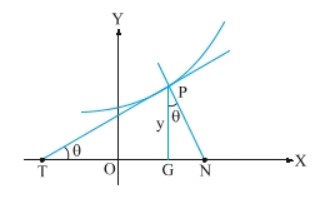
\includegraphics{images/tangentGraph}
\end{figure}
\subsubsection{Length of Subtangent}
Subtangent $= TG = \dfrac{\abs{y}}{\tan(\theta)} = \dfrac{\abs{y}}{\left( \dfrac{\dif y}{\dif x} \right)}$
\subsubsection{Length of Subnormal}
Subnormal $= GN = \abs{y} \tan(\theta) = \abs{y} \dfrac{\dif y}{\dif x}$
\subsubsection{Length of Tangent}
Tangent $= PT = \dfrac{\abs{y}}{\sin(\theta)} = \abs{y} \csc(\theta) = \abs{y} \sqrt{1 + \cot^2(\theta)} = \dfrac{\abs{y} \sqrt{1 + \left(\dfrac{\dif y}{\dif x}\right)^2}}{\abs{\dfrac{\dif y}{\dif x}}}$
\subsubsection{Length of Normal}
Normal $= PN = \abs{y} \sec(\theta) = \abs{y} \sqrt{1 + \tan^2(\theta)} = \abs{y} \sqrt{1 + \left(\dfrac{\dif y}{\dif x}\right)^2}$
\subsubsection{Length of the Curve from $a$ to $b$}
Length of curve = $\bigints\limits_a^b \left(1 + \left(\dfrac{\dif y}{\dif x}\right)^2\right) \dif x$
\subsubsection{Radius of Curvature}
$R = \dfrac{\left[ 1 + \left(\dfrac{\dif y}{\dif x}\right)^2\right]^{\dfrac32}}{\dfrac{\dif^{\;2}y}{\dif x ^2}}$
\pagebreak
\subsection{Local Maxima and Minima}
\subsubsection{Local Maximum}
\begin{define}
Let a function $f$ be defined on a set $S$. The point $c \in S$ is called a \underline{point of local maximum} if there exists an open interval $I$ containing $c$ such that $f(c) \geq f(x) \forall x \in I \cap S$ and $I$ should be a subset of $S$.
\end{define}
\subsubsection{Local Minimum}
\begin{define}
Let a function $f$ be defined on a set $S$. The point $c \in S$ is called a \underline{point of local minimum} if there exists an open interval $I$ containing $c$ such that $f(c) \leq f(x) \forall x \in I \cap S$ and $I$ should be a subset of $S$.
\end{define}
Note that Local Maxima and Local Minima don't exist at end-points because you can't have an open interval which contains the end-point and is a subset of $S$.
\subsection{Fermat's Theorem}
\begin{theorem}
If a function attains a local maximum or a local minimum at an interior point $c$, and if the function is differentiable at $c$, then $f'(c) = 0$.
\end{theorem}
\subsection{Rolle's Theorem}
\begin{theorem}
If a function $f$ is continuous in $[a, b]$ and differentiable in $(a, b)$ and $f(a) = f(b)$, then there exists at least one $c \in (a, b)$ such that $f'(c) = 0$.
\end{theorem}
\subsubsection{Conclusions}
Let $f$ be a function which is infinitely continuously differentiable (i.e. all subsequent derivatives are also continuous), then:
\begin{itemize}
\item Between two real roots of $f(x) = 0$ lies at least one real root of $f'(x) = 0$.
\item Between $n$ real roots of $f(x) = 0$ lie at least $(n - 1)$ real roots of $f'(x) = 0$
\item Between $n$ real roots of $f(x) = 0$ lie at least $(n - 2)$ real roots of $f''(x) = 0$\\
(Generalizing)
\item Between $n$ real roots of $f(x) = 0$ lie at least $(n - k)$ real roots of $f^{(k)}(x) = 0$
\item If $f^{(k)}(x) = 0$ has $(n - k)$ roots, then $f(x) = 0$ has at most $n$ roots.
\end{itemize}
\subsection{Linear Differential Equation and Inequality}
\[f'(x) + k f(x) = 0\]
\[f'(x) - k f(x) = 0\]
Whenever we see an equation or inequality of this form, we will multiply both sides by the integrating factor. The integrating factor of $f'(x) + k f(x)$ is ${\rm e}^{kx}$ and that of $f'(x) - k f(x)$ is ${\rm e}^{-kx}$. Notice that both are positive and won't change the sign of the inequality.
\begin{align*}
{\rm e}^{kx}f'(x) + k {\rm e}^{kx} f(x) = 0\\
\dfrac{\dif}{\dif x}\left({\rm e}^{kx} f(x)\right) = 0
\end{align*}
\pagebreak
\subsection{Darboux's Theorem}
\begin{theorem}
If a function $f$ is differentiable in the closed interval $I = [a, b]$ and $f'(a) < k < f'(b)$, then $\exists \; c \in (a, b) : f'(c) = k$.\\
In other words, $f'(x)$ will have intermediate value property.
\end{theorem}
\subsection{Multiplicity of Roots and Rolle's Theorem}
Suppose $f$ is a polynomial of which $\alpha$ is a zero with multiplicity $r$ where $f(x) = (x-\alpha)^r \cdot g(x)$, where $g$ is another polynomial and $g(\alpha) \neq 0$. Then $f'(x)$ has $\alpha$ as one of its zeros with multiplicity $(r - 1)$.
\begin{proof}
\begin{align*}
f(x) &= (x - \alpha)^r \cdot g(x)\\
f'(x) &= r(x - \alpha)^{r-1}\cdot g(x) + (x - \alpha)^r \cdot g'(x)\\
&= (x - \alpha)^{r-1} \left[ r g(x) + (x - \alpha) g'(x) \right]
\end{align*}
Now, observing $\left[ r g(x) + (x - \alpha) g'(x) \right]$. This won't be zero at $x = \alpha$ since $g(\alpha) \neq 0$ [given].\\
Also, $(x - \alpha)^{r-1}$ has $\alpha$ as a zero with multiplicity $(r - 1)$.\\
Therefore, $f'(x)$ will have $\alpha$ as one of its zeros with multiplicity $(r - 1)$.\\
\end{proof}
Similarly, the multiplicity of $\alpha$ in $f''(x)$ will be $(r - 2)$ and so on...\\
The converse is also true.
\pagebreak
\subsection{Problems on Rolle's Theorem and Roots}
\begin{prob}
Prove that $x {\rm e}^x = 1$ has exactly one root in $(0, 1)$.
\begin{proof}
Consider a function $f(x) = x {\rm e}^x - 1$.\\
We need to prove that $f(x)$ has at least one root in $(0, 1)$.\\
Now, $f$ is continuous everywhere, so it's also continuous in $[0, 1]$.\\
Applying Bolzano's Theorem:
\begin{align*}
f(0) &= 0 - 1 = -1 < 0\\
f(1) &= {\rm e} - 1 > 0\\
\Rightarrow f(0) \cdot f(1) &< 0
\end{align*}
Therefore, there exists \textbf{at least one} root of $f(x)$ in $(0, 1)$.\\
But we have to prove that it has exactly one root.\\
Assume for the purpose of contradiction that $f(x)$ has two roots in $(0, 1)$.\\
Then by Rolle's theorem, $f'(x)$ will have at least one root in $(0, 1)$.\\
\begin{equation*}
f'(x) = {\rm e} ^ x + x {\rm e}^x
\end{equation*}
But ${\rm e} ^ x + x {\rm e}^x > 0 \; \forall x \in (0, 1)$\\
Or, $f'(x)$ has no root in $(0, 1)$.\\ This contradicts our assumption that $f(x)$ has two roots in $(0, 1)$.\\
$\therefore f$ has exactly one root in (0, 1). 
\end{proof}
\end{prob}
\begin{prob}
Comment on the number of roots of $f(x) = x^4- 4x - 1$.\\
\textbf{Solution: } The given polynomial is of even degree and has the leading coefficient and constant term of opposite signs. Therefore it has at least 2 real roots: one in $(-\infty, 0)$ and the other in $(0, \infty)$.\\
Assume $f(x)$ has 3 or more roots.\\
Then $f'(x)$ should have at least 2 real roots.\\
\begin{align*}
f'(x) &= 4x^3 - 4\\
&= 4(x^3 - 1)
\end{align*}
But $f'(x)$ has exactly 1 real root (i.e. $x = 1$). This is a contradiction.\\
Therefore, $f(x)$ has exactly 2 roots.
\end{prob}
\pagebreak
\begin{prob}
Let $f$ be a function which is differentiable on $\mathbb{R}$ and $\alpha$ and $\beta$ be two numbers such that $\alpha < \beta$ and $f(\alpha) = f(\beta) = 0$. Then which of the following is/are correct?\\
\begin{enumerate*}[label=(\Alph*)]
\item There exists $c \in (\alpha, \beta)$ such that $f'(c) = f(c)$\\
\item There exists $c \in (\alpha, \beta)$ such that $f'(c) = 2f(c)$\\
\item There exists $c \in (\alpha, \beta)$ such that $f'(c) = 3f(c)$\\
\item There exists $c \in (\alpha, \beta)$ such that $f'(c) = kf(c)$ for any real $k$\\
\end{enumerate*}\\
\textbf{Solution: (A, B, C, D) } D is just a generalization of A, B and C. So if we prove D, that will prove all the options.\\
We have to prove that $\exists c \in (\alpha, \beta) \mid f'(c) - kf(c) = 0 \;\forall k > 0$\\
Consider $g(x) = {\rm e}^{-kx} f(x)$\\
$g$ is continuous in $[a, b]$ and differentiable in $(a, b)$\\
Now, $g(\alpha) = 0$ and $g(\beta) = 0$ because $f(\alpha) = f(\beta) = 0$ [Given]\\
Then by Rolle's Theorem,
\begin{align*}
\exists c \in (\alpha, \beta) : g'(c) &= 0\\
\Rightarrow {\rm e}^{-kc} f'(c) - k{\rm e}^{-kc}f(c) &= 0 && \text{Divide by } {\rm e}^{-kc}\\
\Rightarrow f'(c) - k f(c) &= 0\\
\Rightarrow f'(c) &= kf(c)
\end{align*}
This completes the proof. Hence all the options \textbf{A, B, C and D} are correct.
\end{prob}
\begin{prob}
If $\dfrac{a}{3} + \dfrac{b}{2} + c = 0$, then prove that the equation $ax^2 + bx + c = 0$ has at least one root in $(0, 1)$
\end{prob}
\begin{proof}
We will treat $ax^2 + bx + c$ as the derivative of some function.\\
Let $f(x) = \dfrac{ax^3}{3} + \dfrac{bx^2}{2} + cx$.
\begin{align*}
f'(x) &= ax^2 + bx + c\\
f(x) &= \dfrac{ax^3}{3} + \dfrac{bx^2}{2} + cx\\
f(1) &= \dfrac{a}3 + \dfrac{b}2 + c = 0\\
f(0) &= 0
\end{align*}
Since $f(x)$ is continuous in $[0, 1]$ and differentiable in $(0, 1)$, Applying Rolle's Theorem,\\
\begin{align*}
\Rightarrow \exists k \in (0, 1) : f'(k) &= 0\\
\Rightarrow \exists k \in (0, 1) : ak^2 + bk + c &= 0
\end{align*}
i.e. $ax^2 + bx + c = 0$ has at least one root in $(0, 1)$
\end{proof}
\pagebreak
\begin{prob}
The Legendre Polynomial is defined by the following formula (Rodrigues Formula).
\[P_n(x) = \dfrac{1}{2^n n!} \dfrac{\dif^{\;n}}{\dif x^n} (x^2 - 1)^n\]
Prove that $P_n(x)$ has $n$ different real roots, all of which are found between $-1$ and $1$.
\begin{proof}
Notice that $\dfrac{1}{2^n n!}$ is just a constant. So the roots of $P_n(x)$ will be the same as the roots of $\dfrac{\dif^{\;n}}{\dif x^n} (x^2 - 1)^n$.\\
Consider $g(x) = (x^2 - 1)^n$. This is a polynomial of degree $2n$. If we differentiate it $n$ times, we will get a polynomial of degree $n$.\\
So $\dfrac{\dif^{\;n}}{\dif x^n} (x^2 - 1)^n$ is a polynomial of degree $n$.
By the Fundamental Theorem of Algebra, it will have at most $n$ roots.\\
\begin{align*}
g(x) &=  (x^2 - 1)^n\\
&= (x+1)^n(x-1)^n
\end{align*}
$g(x)$ has two roots: $-1$ and $1$, each having multiplicity $n$.\\\\
By Rolle's Theorem, $g'(x)$ will have at least one root in $(-1, 1)$. Also $g'(x)$ will have $-1$ and $1$ as roots, each having multiplicity $(n-1)$. So $g'(x)$ has at least $3$ distinct roots.\\\\
Again applying Rolle's Theorem, between 3 roots of $g'(x)$ will lie at least 2 real roots of $g''(x)$. And $g''(x)$ will have $-1$ and $1$ as roots of multiplicity $(n-2)$. So $g''(x)$ will have at least $4$ distinct roots.\\\\
And so on...\\\\
Applying Rolle's Theorem $(n-1)$ times. Then $g^{(n-1)}(x)$ will have at least $n-1$ roots in $(0, 1)$ and also $-1$ and $1$ as roots of multiplicity $1$ each. So $g^{(n-1)}(x)$ will have at least $(n + 1)$ real roots.\\\\
\begin{figure}[h]
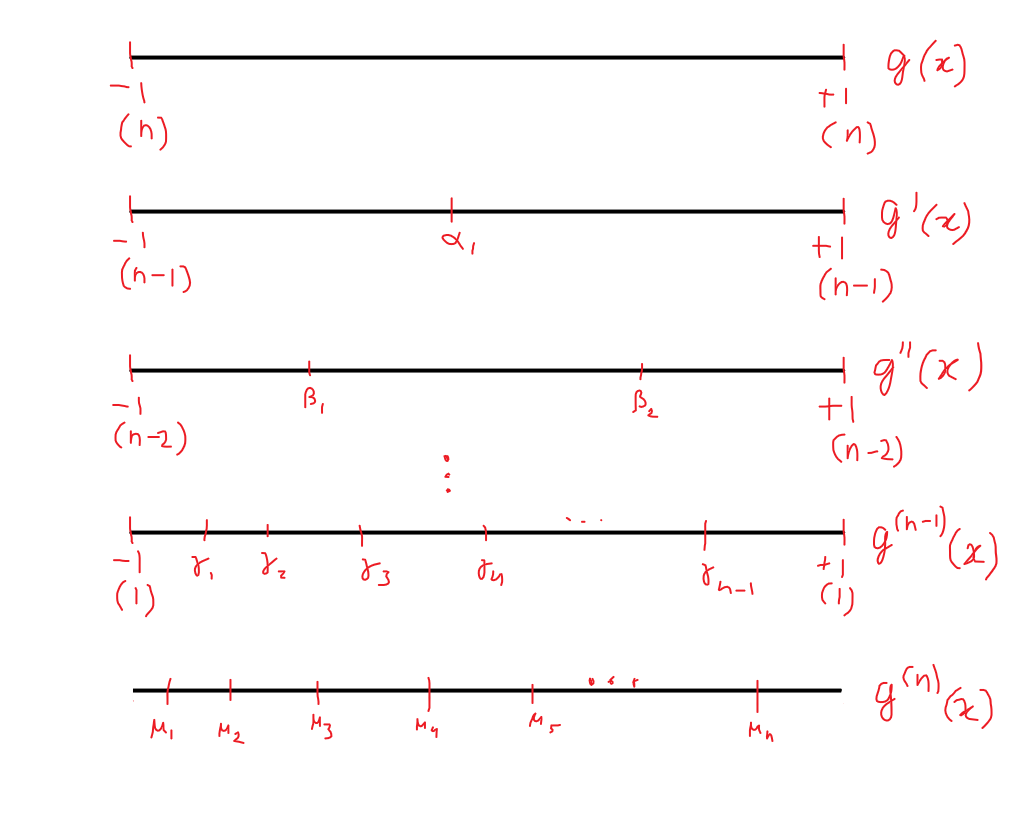
\includegraphics[scale=0.35]{images/legendre}
\end{figure}
Finally, applying Rolle's Theorem, $g^{(n)}(x)$ will have at least $n$ roots, all of which lie in $(0, 1)$.\\
Therefore, $P_n(x)$ will have exactly $n$ real roots, all of which lie in $(0, 1)$
\end{proof}
\end{prob}
\pagebreak
\subsection{Mean Value Theorems}
\subsubsection{Lagrange's Mean Value Theorem}
\begin{theorem}
If a function $f$ is continuous in $[a, b]$ and differentiable in $(a, b)$, then there exists at least one $c \in (a, b)$ such that:
\[\dfrac{f(b) - f(a)}{b - a} = f'(c)\]
Geometrically, it means at that at some point in the interval $(a, b)$, the tangent will be parallel to the chord.
\end{theorem}
\begin{proof}
Consider the following function.
\[g(x) = \left( f(b) - f(a) \right)x - f(x)\cdot (b - x)\]
Then,
\[g'(x) = f(b) - f(a) - f'(x) \cdot (b - a)\]
Now, $g$ is continuous in $[a, b]$ and differentiable in $(a, b)$ and $g(a) = g(b)$. Applying Rolle's Theorem.\\
$\exists c \in (a, b)$ such that $g'(c) = 0$.\\
\begin{align*}
\Rightarrow f(b) - f(a) - f'(c) \cdot (b - a) &= 0\\
\Rightarrow f(b) - f(a) &= f'(c) \cdot (b - a)\\
\Rightarrow \dfrac{f(b) - f(a)}{b - a} &= f'(c)
\end{align*}
\end{proof}
\subsubsection{Cauchy's Mean Value Theorem}
\begin{theorem}
Let $f$ and $g$ be two functions continuous in $[a, b]$ and differentiable in $(a, b)$, then there exists at least one $c \in (a, b)$ such that $\dfrac{f(b) - f(a)}{g(b) - g(a)} = \dfrac{f'(c)}{g'(c)}$
\end{theorem}
\begin{proof}
We need to prove that for some $x = c$, where $c \in (a, b)$, $\dfrac{f(b) - f(a)}{g(b) - g(a)} = \dfrac{f'(x)}{g'(x)}$.\\
Or $g'(x) \cdot \left( f(b) - f(a) \right) - f'(x) \cdot \left( g(b) - g(a) \right) = 0$.
Consider the following function:
\[h(x) = g(x) \cdot \left( f(b) - f(a) \right) - f(x) \cdot \left( g(b) - g(a) \right)\]
Then,
\[h'(x) = g'(x) \cdot \left( f(b) - f(a) \right) - f'(x) \cdot \left( g(b) - g(a) \right)\]
Now, $h(x)$ is  continuous in $[a, b]$ and differentiable in $(a, b)$ and $h(a) = h(b)$. Applying Rolle's Theorem.\\
$\exists c \in (a, b)$ such that $h'(c) = 0$\\
Or $g'(c) \cdot \left( f(b) - f(a) \right) - f'(c) \cdot \left( g(b) - g(a) \right) = 0$\\
$\Rightarrow \dfrac{f(b) - f(a)}{g(b) - g(a)} = \dfrac{f'(c)}{g'(c)}$\\
\end{proof}
\pagebreak
\subsubsection{Important Result from Lagrange's Mean Value Theorem}
\begin{theorem}
If $f'(x) > g'(x) \; \forall x$ and $f(a) = g(a)$, then $f(x) > g(x) \; \forall x > a$ and $f(x) < g(x) \; \forall x < a$.
\end{theorem}
\begin{proof}
Consider $h(x) = f(x) - g(x)$\\
Then $h'(x) = f'(x) - g'(x)$\\
Also, $h'(x) > 0 \; \forall x$\\
Then we have to prove that $h(x) > 0 \; \forall x > a$ and $h(x) < 0 \; \forall x < a$.\\
Now,
\begin{align*}
h(a) = f(a) - g(a) = 0 && \because f(a) = g(a) \text{ [given]}
\end{align*}
Consider any real number $x \neq a$.\\
Note that $h$ is continuous and differentiable. Applying Lagrange's Mean Value Theorem.
\[\exists c : \dfrac{h(x) - h(a)}{x - a} = h'(c) > 0\]
\textbf{Case 1:} $x > a$\\
Then $x - a > 0$,\\
Therefore,\\
\[h(x) - h(a) > 0\]
\[\Rightarrow h(x) > h(a)\]
\textbf{Case 2:} $x < a$\\
Then $x - a < 0$,\\
Therefore,\\
\[h(x) - h(a) < 0\]
\[\Rightarrow h(x) < h(a)\]
\end{proof}
\pagebreak
\subsubsection{Example Problems}
\begin{prob}
Suppose $f'(x) \geq M$ in the interval $[a, b]$, then prove that $f(b) \geq f(a) + M(b - a)$
\end{prob}
\begin{proof}
$f(x)$ is continuous in $[a, b]$ and differentiable in $(a, b)$.\\
Applying Lagrange's Mean Value Theorem.
\[\exists c \in (a, b) : \dfrac{f(b) - f(a)}{b - a} = f'(c)\]
But $f'(x) \geq M \; \forall x \in [a, b]$ (Given), so\\
\begin{align*}
\dfrac{f(b) - f(a)}{b - a} &\geq M\\
f(b) - f(a) &\geq M (b - a)\\
f(b) &\geq f(a) + M (b - a)
\end{align*}
\end{proof}
\begin{prob}
Suppose $f'(x) \leq M$ in the interval $[a, b]$, then prove that $f(b) \leq f(a) + M(b - a)$
\end{prob}
\begin{proof}
$f(x)$ is continuous in $[a, b]$ and differentiable in $(a, b)$.\\
Applying Lagrange's Mean Value Theorem.
\[\exists c \in (a, b) : \dfrac{f(b) - f(a)}{b - a} = f'(c)\]
But $f'(x) \leq M \; \forall x \in [a, b]$ (Given), so\\
\begin{align*}
\dfrac{f(b) - f(a)}{b - a} &\leq M\\
f(b) - f(a) &\leq M (b - a)\\
f(b) &\leq f(a) + M (b - a)
\end{align*}
\end{proof}
\begin{prob}
Let the second derivative $f''$ of a function be continuous and satisfy $\abs{f''(x)} \leq 1$. If $f(0) = f(1)$, show that $\abs{f'(x)} < 1 \;\forall x \in (0, 1)$.
\end{prob}
\begin{proof} $\text{}$\\
$f$ is continuous in $[0, 1]$ and differentiable in $(0, 1)$, and $f(0) = f(1)$. Applying Rolle's Theorem.\\
$\exists c \in (0, 1) : f'(c) = 0$ or $\abs{f'(c)} \leq 1$\\
But we have to prove it for all $x$ not just some specific value.\\
\textbf{General advice:} If you see an inequality in the second derivative, using Lagrange's Mean Value Theorem could be helpful.\\
Applying Lagrange's Mean Value Theorem.\\
Consider any $x \in (0, 1) - \{c\}$.\\
The function $f'$ is continuous in $[x, c]$ or $[c, x]$ and differentiable in $(x, c)$ or $(c, x)$
\[\dfrac{f'(x) - f'(c)}{x - c} = f''(c_1) \text{\; for some } c_1 \in (x, c) \text{ or } (c, x)\]
\[\abs{f'(x) - f'(c)} = \abs{x - c} \cdot \abs{f''(c_1)} \;\; [\text{Now, } f'(c) = 0 \text{ and } \abs{f''(c_1)} \leq 1 ]\]
\[\abs{f'(x)} = \abs{x - c} \cdot \abs{f''(c_1)} \leq \abs{x - c} < 1\]
\end{proof}
\pagebreak
\begin{prob}
Assume that $\abs{f''(x)} \leq m$ for each $x$ in the interval $[0, a]$ and assume that $f$ takes its largest value at an interior point in this interval. If $f''$ is continuous in the closed interval $[0, a]$, show that $\abs{f'(0)} + \abs{f'(a)}\leq am$ where $f'(0)$ denotes the right-hand derivative of $f$ at $0$ and $f'(a)$ denotes the left-hand derivative of $f$ at $a$.
\end{prob}
\begin{proof}
$f$ takes its largest value at an interior point of $[0, a]$.\\
Or, $f$ has a point of maximum in $(0, a)a$.\\
By Fermat's Theorem, \[\exists c \in (0, a) : f'(c) = 0\]\\
Applying Lagrange's Mean Value Theorem on $f'$ in $[0, c]$.\\
\[\dfrac{f'(0) - f'(c)}{0 - c} = f''(c_1) \text{\;\;\; for some } c_1 \in (0, c)\]
But $f'(c) = 0$\\
Taking modulus on both sides and multiplying by $\abs{c}$
\[\abs{f'(0)} = \abs{c} \cdot \abs{f''(c_1)}\]
But $\abs{f''(c_1)}\leq m$
\begin{equation}\label{eqn:c1}
\abs{f'(0)} = \abs{c} \cdot \abs{f''(c_1)} \leq \abs{c} \cdot m
\end{equation}
Applying Lagrange's Mean Value Theorem on $f'$ in $[c, a]$.\\
\[\dfrac{f'(a) - f'(c)}{a - c} = f''(c_2) \text{\;\;\; for some } c_2 \in (c, a)\]
But $f'(c) = 0$
Taking modulus on both sides and multiplying by $\abs{a - c}$
\[\abs{f'(a)} = \abs{a - c} \cdot \abs{f''(c_2)}\]
But $\abs{f''(c_2)} \leq m$
\begin{equation}\label{eqn:c2}
\abs{f'(a)} = \abs{a - c} \cdot \abs{f''(c_2)} \leq \abs{a - c} \cdot m
\end{equation}
Adding $(\ref{eqn:c1})$ and $(\ref{eqn:c2})$,
\begin{align*}
\abs{f'(0)} + \abs{f'(a)} &\leq \abs{c} \cdot m + \abs{a - c} \cdot m\\
\abs{f'(0)} + \abs{f'(a)} &\leq m \cdot \left(\abs{c} + \abs{a - c}\right)\\
\abs{f'(0)} + \abs{f'(a)} &\leq m \cdot \abs{a} && \text{But } a \geq 0 \text{ so } \abs{a} = a \\
\Rightarrow \abs{f'(0)} + \abs{f'(a)} &\leq a m
\end{align*}
\end{proof}
\pagebreak
\begin{prob}
Suppose $f$ is continuous on $[a, b]$ and differentiable on $(a, b)$. Assume further that $f(b) - f(a) = b - a$, then prove that for all positive integer $n$, there exist distinct points $c_1, c_2, c_3, \cdots, c_n$ such that $f'(c_1) + f'(c_2) + f'(c_3) + \cdots + f'(c_n) = n$.
\end{prob}
\begin{proof}
We will try to prove it for $n = 1$ and $n = 2$, and then we'll try to draw inspiration from it to prove for any general $n$.\\
\textbf{For $n = 1$,}\\
$f$ is continuous in $[a, b]$ and differentiable in $(a, b)$.\\
Applying Lagrange's Mean Value Theorem.\\
\[
\exists c_1 \in (a, b) : \dfrac{f(b) - f(a)}{b - a} = f'(c_1)
\]
But $f(b) - f(a) = b - a$ (Given),
\begin{align*}
\Rightarrow\exists c_1 \in (a, b) &: \dfrac{\cancel{b - a}}{\cancel{b - a}} = f'(c_1)\\
\Rightarrow\exists c_1 \in (a, b) &: f'(c_1) = 1
\end{align*}
And this proves the result for $n = 1$.\\
\textbf{For $n = 2$,}\\
We need to prove that there exist $c_1$ and $c_2$ such that $f'(c_1) + f'(c_2) = 2$
We will divide the interval $[a, b]$ into $2$ equal parts using the point $\dfrac{a + b}{2}$.\\
Applying Lagrange's Mean Value Theorem and Adding the equations.\\
For some $c_1$ and $c_2$,
\begin{align*}
\cancel{f\left(\dfrac{a+b}{2}\right)} - f(a) &= \dfrac{b-a}{2} f'(c_1)\\
f(b) - \cancel{f\left(\dfrac{a+b}{2}\right)} &= \dfrac{b - a }{2} f'(c_2)\\
\cline{0-1}
f(b) - f(a) &= \dfrac{b - a}{2} \left(f'(c_1) + f'(c_2)\right)\\
\cline{0-1}
\end{align*}
$\Rightarrow \dfrac{f(b) - f(a)}{b - a} = \dfrac12 \left(f'(c_1) + f'(c_2)\right)$\\
But $f(b) - f(a) = b - a$ (Given),
\[\Rightarrow \dfrac{\cancel{b - a}}{\cancel{b - a}} = \dfrac12 \left(f'(c_1) + f'(c_2)\right) \]
\[f'(c_1) + f'(c_2) = 2\]
This proves the result for $n = 2$.
\pagebreak
Now we will prove it for any general $n$ by the same analogy.\\\\
\textbf{For any General $n$,}\\
For the case of $n = 2$, we divided the interval $(a, b)$ into two equal parts.\\
So for the general case, we will try to divide the interval into $n$ equal parts, i.e. $\left(a, a + \dfrac{b - a}{n}\right),\\ \left(a + \dfrac{b - a}{n}, a + \dfrac{2(b - a)}{n}\right), \left(a + \dfrac{2(b - a)}{n}, a + \dfrac{3(b - a)}{n}\right), \cdots, \left(a + \dfrac{(n-1)(b - a)}{n}, b\right)$\\\\
Applying Lagrange's Mean Value Theorem $n$ times (on each of these intervals) and adding all the resulting equations. This makes a telescopic sum. There exist $c_1, c_2, c_3, \cdots, c_n$ such that:
\begin{align*}
\cancel{f\left(a + \dfrac{b - a}{n}\right)} - f(a) &= \left(\dfrac{b - a}{n}\right) \cdot f'(c_1)\\
\cancel{f\left(a + \dfrac{2(b - a)}{n}\right)} - \cancel{f\left(a + \dfrac{b - a}{n}\right)} &= \left(\dfrac{b - a}{n}\right) \cdot f'(c_2)\\
\cancel{f\left(a + \dfrac{3(b - a)}{n}\right)} - \cancel{f\left(a + \dfrac{2(b - a)}{n}\right)} &= \left(\dfrac{b - a}{n}\right) \cdot f'(c_3)\\
\cancel{f\left(a + \dfrac{3(b - a)}{n}\right)} - \cancel{f\left(a + \dfrac{2(b - a)}{n}\right)} &= \left(\dfrac{b - a}{n}\right) \cdot f'(c_3)\\
\cancel{f\left(a + \dfrac{4(b - a)}{n}\right)} - \cancel{f\left(a + \dfrac{3(b - a)}{n}\right)} &= \left(\dfrac{b - a}{n}\right) \cdot f'(c_4)\\
\vdots\;\;\;\;\;\;\;\;\;\;\;\;\;\;\;\;\;\;\;\;\;\;\;\;\vdots\;\;\;\;\;\;\;\;\;\;\;\;\;&= \;\;\;\;\;\;\;\;\vdots\\
f\left(b \right) - \cancel{f\left(a + \dfrac{(n-1)(b - a)}{n}\right)} &= \left(\dfrac{b - a}{n}\right) \cdot f'(c_n)\\
\cline{0-1}
f(b) - f(a) &= \left(\dfrac{b-a}{n}\right)\cdot \left(f'(c_1) + f'(c_2) + \cdots + f'(c_n)\right)\\
\cline{0-1}
\end{align*}
$\Rightarrow \dfrac{f(b) - f(a)}{b - a} =\dfrac1{n} \left(f'(c_1) + f'(c_2) + \cdots + f'(c_n)\right)$\\\\
But $f(b) - f(a) = b - a$
\begin{align*}
\Rightarrow \dfrac{\cancel{b - a}}{\cancel{b - a}} =\dfrac1{n} \left(f'(c_1) + f'(c_2) + \cdots + f'(c_n)\right)\\
\Rightarrow f'(c_1) + f'(c_2) + f'(c_3) + \cdots + f'(c_n) = n
\end{align*}
\end{proof}
\pagebreak
\subsubsection*{Proving Some Inequalities}
\begin{prob}
Prove that $\forall a, b \in \mathbb{R}$, 
\[\abs{\sin(a) - \sin(b)} \leq \abs{a - b}\]
\end{prob}
\begin{proof} (using Lagrange's Mean Value Theorem)\\
\textbf{Case 1:} If $a = b$\\
This inequality is trivially true if $a = b$, because $LHS = \sin(a) - \sin(a) = 0$ and $RHS = a - a = 0$\\\\
\textbf{Case 2:} If $a \neq b$\\
Consider a function $f(x) = \sin(x)$
$f$ is continuous and differentiable everywhere. Applying Lagrange's Mean Value Theorem.\\
There exists $c \in (a, b)$ or $(b, a)$ such that
\begin{align*}
\dfrac{\sin(a) - \sin(b)}{a - b} &= \cos(c)\\
\Rightarrow \abs{\dfrac{\sin(a) - \sin(b)}{a - b}} &= \abs{\cos(c)} \leq 1 && \text{Multiply by } \abs{a - b}\\
\Rightarrow \abs{\sin(a) - \sin(b)} &\leq \abs{a - b}
\end{align*}
\end{proof}
\begin{prob}
Prove that $\forall x > 0$,
\[\dfrac{x}{1+x} < \log_{\rm e}(1+x) < x\]
\end{prob}
\begin{proof}
Consider the function $f(t) = \log_{\rm e}(t)$\\
$f$ is continuous in $[1, 1+x]$ and differentiable in $(1, 1+x)$. Applying Lagrange's Mean Value Theorem.\\
There exists $c \in (1, 1 + x)$ such that
\[\dfrac{\ln(1 + x) - \ln(1)}{1 + x - 1} = \dfrac1{c}\]
Now,
\[1 < c < 1+x\]
\[\Rightarrow \dfrac1{1 + x} < \dfrac1{c} < 1\]
\[\Rightarrow \dfrac1{1 + x} < \dfrac{\ln(1 + x) - \ln(1)}{\cancel{1} + x \cancel{- 1}} < 1\]
But $\ln(1) = 0$
\[\Rightarrow \dfrac1{1 + x} < \dfrac{\ln(1 + x)}{x} < 1\]
Now, $x > 0$ (Given), so multiplying by x,
\[\dfrac{x}{1 + x} < \ln(1+x) < x\]
\end{proof}
\pagebreak
\begin{prob}
Show that the square roots two successive natural numbers greater than $N^2$ differ by less than $\dfrac1{2N}$.
\end{prob}
\begin{proof}
Consider any two consecutive natural numbers $m$ and $m + 1$, both greater than $N^2$.\\
Also consider the function $f(x) = \sqrt{x}$.\\
Applying Lagrange's Mean Value Theorem,\\
$f(x)$ is continuous in $[m, m + 1]$ and differentiable in $(m, m + 1)$.\\
Therefore, there exists $c \in (m, m+1)$ such that
\begin{align*}
\dfrac{\sqrt{m + 1} - \sqrt{m}}{m + 1 - m} &= f'(c)\\
\sqrt{m + 1} - \sqrt{m} &= \dfrac{1}{2\sqrt{c}}
\end{align*}
Now,
\[m < c < m + 1\]
\[\sqrt{m} < \sqrt{c} < \sqrt{m + 1}\]
\[\dfrac1{\sqrt{m + 1}} < \dfrac{1}{\sqrt{c}} < \dfrac1{\sqrt{m}}\]
Also, it is given that
\[N^2 < m < m + 1\]
\[\Rightarrow N < \sqrt{m} < \sqrt{m + 1}\]
\[\Rightarrow\dfrac1{\sqrt{m + 1}} < \dfrac1{\sqrt{m}} < \dfrac{1}{N}\]
So $\dfrac1{\sqrt{c}} < \dfrac1{\sqrt{m}}$ and $\dfrac{1}{\sqrt{m}} < \dfrac1{N}$
\[\Rightarrow \dfrac1{\sqrt{c}} < \dfrac1{N}\]
Therefore,
\[\sqrt{m + 1} - \sqrt{m} = \dfrac{1}{2\sqrt{c}} < \dfrac{1}{2N}\]
\[\Rightarrow\sqrt{m + 1} - \sqrt{m} < \dfrac{1}{2N}\]
\end{proof}
\end{document}
